% =====================================================================
% Proposta - Edital FAPERJ nº 34/2026 - PROFIX-RJ (FAPERJ/CNPq/CAPES)
% Limite: 20 páginas, incluindo orçamento (Anexo 1, II.II-a)
% A interface com EOR é uma perspectiva de integração futura, não uma meta de validação.
% Itens marcados com \pendente{...} precisam ser preenchidos.
% =====================================================================
\documentclass[10pt,a4paper]{article}

\usepackage[utf8]{inputenc}
\usepackage[T1]{fontenc}
\usepackage[brazil]{babel}
\usepackage{lmodern}
\usepackage[a4paper,margin=1.75cm,headsep=0.35cm]{geometry}
\usepackage{setspace}
\usepackage{xcolor}
\usepackage{graphicx}
\usepackage{booktabs}
\usepackage{tabularx}
\usepackage{longtable}
\usepackage{array}
\usepackage{colortbl}
\usepackage{enumitem}
\usepackage[fleqn]{amsmath}
\setlength{\mathindent}{1em}
\usepackage{amssymb}
\usepackage{siunitx}
\usepackage[version=4]{mhchem}
\usepackage[numbers,sort&compress]{natbib}
\usepackage{xurl}
\usepackage{multicol}
\usepackage[hidelinks]{hyperref}
\usepackage{titlesec}
\titlespacing*{\section}{0pt}{7pt plus 1pt minus 1pt}{3pt}
\titlespacing*{\subsection}{0pt}{5pt plus 1pt minus 1pt}{2pt}
\usepackage{fancyhdr}
\usepackage{tikz}
\usepackage{tocloft}
\setlength{\cftbeforesecskip}{1.5pt}
\renewcommand{\cftsecfont}{\bfseries}
\renewcommand{\cftsecpagefont}{\bfseries}
\renewcommand{\cftdot}{.}
\renewcommand{\cftsecleader}{\cftdotfill{\cftdotsep}}

\setstretch{1.025}
\setlist{noitemsep,topsep=1pt,leftmargin=1.3em}
\renewcommand{\topfraction}{0.9}
\renewcommand{\bottomfraction}{0.8}
\renewcommand{\textfraction}{0.07}
\renewcommand{\floatpagefraction}{0.8}
\setcounter{topnumber}{3}
\sisetup{group-separator={.},output-decimal-marker={,}}

% --- Marcadores ---------------------------------------------------------
\newcommand{\pendente}[1]{\textcolor{red}{\textbf{[PENDENTE: #1]}}}
% Referência ao item do edital: invisível no PDF, mantida no código como guia.
% Para exibir, troque a definição por: \hfill{\footnotesize\textcolor{gray}{(Edital: #1)}}
\newcommand{\itemedital}[1]{}
\newcommand{\X}{\cellcolor{gray!45}}   % célula preenchida no cronograma
\newcolumntype{C}{>{\centering\arraybackslash}X}   % coluna X centralizada

% --- Cabeçalho ----------------------------------------------------------
\pagestyle{fancy}
\fancyhf{}
\lhead{\footnotesize PROFIX-RJ -- FAPERJ/CNPq/CAPES -- 2026}
\rhead{\footnotesize Página \thepage}
\renewcommand{\headrulewidth}{0.4pt}

\titleformat{\section}{\normalsize\bfseries}{\thesection.}{0.5em}{}
\titleformat{\subsection}{\normalsize\bfseries}{\thesubsection}{0.5em}{}

% =====================================================================
\begin{document}

% ---------------------------------------------------------------------
% CAPA
% ---------------------------------------------------------------------
\begin{titlepage}
\pagenumbering{Roman}
\thispagestyle{empty}
\begin{center}
{\large\bfseries UNIVERSIDADE FEDERAL DO RIO DE JANEIRO\\[0.3em]
INSTITUTO ALBERTO LUIZ COIMBRA DE PÓS-GRADUAÇÃO\\ E PESQUISA DE ENGENHARIA -- COPPE\\[0.3em]
PROGRAMA DE ENGENHARIA MECÂNICA -- PEM}

\vspace{0.9cm}
{\normalsize Proposta submetida ao\\[0.3em]
\bfseries Edital FAPERJ nº 34/2026 -- Programa de Apoio à Fixação de Doutores no\\
Estado do Rio de Janeiro -- Conhecimento Brasil / PROFIX-RJ\\
(FAPERJ/CNPq/CAPES)}

\vspace{1.0cm}
{\LARGE\bfseries\setstretch{1.3}
Otimização da composição química da água de injeção baseada em dados geológicos,
geoquímicos e operacionais por algoritmos de aprendizado por reforço e redes
neurais informadas pela física (PINNs) para preservação da injetividade\par}

\vspace{1.0cm}
{\large Proponente: \textbf{Ramon de Paoli Mendes}}
\end{center}

\vfill
\noindent
{\small
\begin{tabularx}{\textwidth}{@{}lX@{}}
\toprule
Instituição executora       & Universidade Federal do Rio de Janeiro (UFRJ) \\
Programa de Pós-Graduação   & Programa de Engenharia Mecânica (PEM) -- COPPE/UFRJ \\
Grande área / área / subárea & Engenharias / Engenharia de Petróleo / \textbf{[confirmar subárea oficial no SisFAPERJ]} \\
Eixo estratégico            & Óleo e gás \\
Bolsa CAPES pleiteada       & Doutorado (48 meses) \\
Duração                     & 48 meses (+3 meses para indicação dos bolsistas CAPES) \\
Auxílio FAPERJ solicitado   & R\$ 200.000,00 \\
\bottomrule
\end{tabularx}}

\vspace{0.5cm}
\begin{center}
Rio de Janeiro\\
Novembro de 2026
\end{center}
\end{titlepage}

% ---------------------------------------------------------------------
% SUMÁRIO
% ---------------------------------------------------------------------
\setcounter{page}{2}
{\setstretch{1.0}\small
\renewcommand{\contentsname}{Sumário}
\tableofcontents\thispagestyle{fancy}}
\clearpage

% ---------------------------------------------------------------------
% NOMENCLATURA
% ---------------------------------------------------------------------
\section*{Nomenclatura}
{\footnotesize\setstretch{1.0}
\renewcommand{\arraystretch}{0.98}
\titlespacing*{\subsection}{0pt}{5pt}{3pt}

\subsection*{Símbolos latinos}
\begin{tabularx}{\textwidth}{@{}p{0.17\textwidth}X@{}}
$a_t$ & Ação no período $t$ (composição, tratamento, dosagens, vazão e temperatura) \\
$c$ & Concentração de partículas em suspensão [m$^3$/m$^3$] \\
$c_i$ & Coeficiente de sensibilidade da grandeza de entrada $x_i$ \\
$c_{\mathrm{trat}},\,c_{\mathrm{bomb}},\,c_{\mathrm{int}}$ & Custos de tratamento, de bombeamento e de intervenção na recompensa \\
$C_{\mathrm{Ba}},\,C_{\mathrm{SO_4}}$ & Concentrações de \ce{Ba^2+} e \ce{SO4^2-} [mol/kg] \\
$\Delta C_{prec}$ & Quantidade precipitada no passo de tempo [mol/kg] \\
$d_t$ & Dano acumulado e sua distribuição radial \\
$\mathcal{D}$ & Conjunto de dados experimentais e de campo \\
$E_n$ & Erro normalizado (ISO 13528) \\
$g_k$ & Restrições operacionais e de segurança \\
$I,\,I_0$ & Índice de injetividade atual e inicial [m$^3$/(s$\cdot$Pa)] \\
$k,\,k_0$ & Permeabilidade atual e inicial [m$^2$]; ($k$ de abrangência em $U = k\,u_c$ é distinto) \\
$K_{sp}$ & Produto de solubilidade do \ce{BaSO4} \\
$L$ & Comprimento do meio poroso [m] \\
$\mathcal{L}$ & Função de perda da PINN (termos de dados, EDP e contorno) \\
$o_t$ & Condições operacionais no período $t$ (pressões, temperatura, pressão do reservatório) \\
$p(\theta\mid\mathcal{D})$ & Distribuição \textit{a posteriori} dos parâmetros dado $\mathcal{D}$ \\
$\Delta P,\,\Delta P_0$ & Sobrepressão de injeção atual e inicial [Pa] \\
$r_t$ & Recompensa no período $t$ \\
$R^2$ & Coeficiente de determinação \\
$s_t$ & Estado do sistema no período $t$ \\
$SR$ & Razão de saturação \\
$t,\,\Delta t$ & Tempo e passo de tempo [s] \\
$T$ & Horizonte de decisão \\
$u$ & Velocidade de Darcy [m/s] \\
$\hat{u}(x,t)$ & Campos aproximados pela PINN (concentração, depósito e pressão) \\
$u_A,\,u_B,\,u_{\mathrm{mod}},\,u_c$ & Incertezas padrão tipo A, tipo B, de modelo e combinada \\
$U$ & Incerteza expandida \\
$w_t$ & Composição das águas disponíveis no período $t$ \\
$x$ & Coordenada espacial [m] \\
$x_{eq}$ & Quantidade termodinamicamente precipitável [mol/kg] \\
\end{tabularx}

\subsection*{Símbolos gregos}
\begin{tabularx}{\textwidth}{@{}p{0.17\textwidth}X@{}}
$\alpha$ & Razão de injetividade, $\alpha = I/I_0 = \Delta P_0/\Delta P$ \\
$\alpha_{\min}$ & Razão de injetividade mínima antes de intervenção \\
$\beta_p,\,\beta_{\mathrm{BaSO_4}}$ & Coeficientes de dano à formação por partículas e por \ce{BaSO4} \\
$\gamma_{\mathrm{Ba}},\,\gamma_{\mathrm{SO_4}}$ & Coeficientes de atividade iônica \\
$\gamma$ & Fator de desconto da recompensa (sem subscrito) \\
$\theta$ & Propriedades da rocha e do poço e parâmetros do dano \\
$\lambda$ & Coeficiente de filtração [1/m] \\
$\lambda_d,\,\lambda_r,\,\lambda_b$ & Pesos dos termos da perda da PINN \\
$\mu$ & Viscosidade da água [Pa$\cdot$s] \\
$\pi$ & Política do agente de RL \\
$\sigma_p,\,\sigma_{\mathrm{BaSO_4}}$ & Volume retido de partículas e de \ce{BaSO4} por volume de rocha \\
$\tau,\,\tau_{prec}$ & Tempo característico de precipitação [s] \\
$\phi,\,\phi_0$ & Porosidade atual e inicial \\
$\phi_{\mathrm{NN}}$ & Pesos da rede neural \\
\end{tabularx}

\subsection*{Siglas e abreviaturas}
\begin{multicols}{3}
\raggedright
\begin{description}[leftmargin=4.4em,labelwidth=4.2em,labelsep=0.2em,itemsep=0pt,font=\normalfont\bfseries]
\item[ANP] Agência Nacional do Petróleo, Gás Natural e Biocombustíveis
\item[CFL] Número de Courant--Friedrichs--Lewy
\item[COPPE] Instituto Alberto Luiz Coimbra de Pós-Graduação e Pesquisa de Engenharia
\item[CVaR] Valor em risco condicional
\item[DeepONet] Rede de operadores profunda
\item[EDP] Equação diferencial parcial
\item[FAIR] Dados localizáveis, acessíveis, interoperáveis e reutilizáveis
\item[FNO] Operador neural de Fourier
\item[GUM] Guia para a expressão de incerteza de medição
\item[IA] Inteligência artificial
\item[IQM] Média interquartil
\item[LRAP+] Laboratório de Recuperação Avançada de Petróleo
\item[MD] Destilação por membrana
\item[NF] Nanofiltração
\item[PEM] Programa de Engenharia Mecânica
\item[PINN] Rede neural informada por física
\item[PPG] Programa de pós-graduação
\item[PTFE] Politetrafluoroetileno (ePTFE: expandido)
\item[RL] Aprendizado por reforço
\item[SRP] Unidade de remoção de sulfato
\item[UFRJ] Universidade Federal do Rio de Janeiro
\end{description}
\end{multicols}
}
\clearpage
\pagenumbering{arabic}

\section*{Resumo}\itemedital{2.16 II; Anexo 1 B}
\addcontentsline{toc}{section}{Resumo}

A reinjeção de água produzida, isoladamente ou misturada à água do mar tratada, é uma estratégia para a gestão da água e a manutenção da pressão em reservatórios de petróleo. Entretanto, a composição físico-química da água injetada pode comprometer a injetividade por mecanismos de dano à formação que interagem e evoluem ao longo do tempo, incluindo precipitação de incrustações minerais (\ce{BaSO4}, \ce{CaCO3} e \ce{SrSO4}), migração e inchamento de argilas, retenção de partículas e gotículas de óleo, formação de reboco e atividade microbiológica. A intensidade desses fenômenos depende da mineralogia, das propriedades petrofísicas e da estrutura porosa da rocha, da composição das águas de formação, produzida e do mar, bem como das condições operacionais do poço. Apesar dessas interdependências, a especificação da água de injeção frequentemente se apoia em análises de compatibilidade e critérios de tratamento avaliados separadamente, sem incorporar plenamente o caráter cumulativo do dano.

Este projeto tem como objetivo desenvolver e validar uma metodologia computacional híbrida capaz de determinar e atualizar, ao longo da operação, as características físico-químicas e as condições de tratamento da água de injeção que melhor preservem a injetividade, respeitando restrições técnicas, econômicas e de segurança. A metodologia será organizada em sete etapas interdependentes: (i) desenvolvimento de um simulador físico de transporte reativo e evolução do dano à formação, com representação dos mecanismos geoquímicos, de retenção e de alteração da permeabilidade; (ii) análise de sensibilidade global e de identificabilidade para selecionar parâmetros dominantes e orientar os ensaios; (iii) realização de ensaios de \textit{coreflooding} para identificação inversa, por PINNs, dos parâmetros físico-químicos e constitutivos que governam o dano à formação, com calibração do simulador e quantificação das incertezas; (iv) treinamento e validação de modelos substitutos (surrogate model) que reproduzam a resposta dinâmica do simulador com menor custo computacional; (v) treinamento e comparação de algoritmos de aprendizado por reforço (RL) para definir sequencialmente proporções de mistura entre fontes de água, composição iônica, salinidade, níveis de tratamento e condições de injeção, considerando os efeitos futuros das decisões; (vi) desenvolvimento e avaliação de um estimador de estados baseado em redes neurais informadas pela física (PINNs), com assimilação de dados operacionais de pressão, vazão e temperatura, para inferir a evolução dos mecanismos de dano à formação e quantificar as incertezas das estimativas; acoplamento desse estimador ao agente de aprendizado por reforço (RL), de modo que as decisões de composição, tratamento e injeção da água sejam atualizadas dinamicamente conforme o estado estimado do poço; e (vii) Validação experimental independente das políticas de otimização desenvolvidas por RL, mediante aplicação de diferentes sequências de composição e tratamento da água em ensaios de \textit{coreflooding}, comparando seus resultados com estratégias convencionais.

A avaliação incluirá a propagação das incertezas dos parâmetros, testes em cenários geológicos e geoquímicos não utilizados no treinamento e análise estatística do desempenho das políticas. Esperam-se como resultados modelos físicos calibrados, parâmetros de dano com incertezas quantificadas, evidências sobre as vantagens e limitações da otimização adaptativa e um software aberto de apoio à decisão para recomendar composições, tratamentos e condições de injeção específicas a diferentes cenários de reservatório. Como impactos potenciais, destacam-se a redução da perda de injetividade, da demanda energética de bombeamento e da necessidade de intervenções corretivas, favorecendo o reaproveitamento da água produzida e a eficiência operacional de campos petrolíferos. A arquitetura do software preverá, adicionalmente, uma interface modular para futura integração com modelos externos de recuperação de petróleo utilizados pelas operadoras, permitindo considerar esse desempenho como objetivo adicional ou restrição, sem incluí-lo na validação experimental desta proposta.

\noindent\textbf{Palavras-chave:} injetividade; água de injeção; dano à formação; transporte reativo; redes neurais informadas pela física; aprendizado por reforço; otimização dinâmica.

% ---------------------------------------------------------------------
\section{Justificativa e diagnóstico da situação atual}\itemedital{2.16 VIII; Anexo 1 C}

A água produzida é o maior efluente líquido da produção de óleo e gás, com estimativa global superior a 250 milhões de barris por dia e volume crescente à medida que os campos amadurecem \cite{macedonio2014,elbadawy2021}. É uma matriz formada pela água de formação
e, em campos sob injeção, pela própria água injetada após a irrupção \cite{liang2018}. Sua reinjeção, isolada ou misturada à água do mar, é a destinação predominante em campos offshore maduros.

A composição dessa água define sua compatibilidade com o reservatório. Ela reúne
eletrólitos monovalentes (\ce{Na+}, \ce{K+}, \ce{Cl-}), cátions divalentes formadores de
incrustação (\ce{Ca^2+}, \ce{Mg^2+}, \ce{Ba^2+}, \ce{Sr^2+}, \ce{Fe^2+}), ânions como
\ce{SO4^2-} e \ce{HCO3-} e gases dissolvidos como \ce{H2S} e \ce{CO2}
\cite{kamal2018}. Quando a água injetada, rica em sulfato, encontra a água de formação rica
em bário e estrôncio, a mistura ultrapassa o limite de solubilidade e precipita sulfatos,
com destaque para o \ce{BaSO4}, cujo produto de solubilidade da ordem de $10^{-10}$ o
torna praticamente irreversível depois de nucleado \cite{binmerdhah2010,bedrikovetsky2009}.
A esse mecanismo somam-se a cristalização de halita em salmouras hipersalinas
\cite{rocha2001,miri2016}, a transição gipsita--anidrita do \ce{CaSO4} nas zonas de gradiente
térmico \cite{kamalipour2017}, a migração de finos por redução de salinidade
\cite{salinity2021}, a filtração profunda de sólidos e óleo \cite{pangsharma1997} e o dano
associado à atividade bacteriana.

O efeito integrado é a perda progressiva de permeabilidade no entorno do poço, com aumento
do fator de película e queda do índice de injetividade \cite{bedrikovetsky2009,pal2023}.
As consequências operam em três escalas: maior pressão de injeção e consumo elétrico das
bombas; intervenções corretivas (acidificação, \textit{scale squeeze}, \textit{workover})
que retiram o poço de serviço e nem sempre restauram a permeabilidade original
\cite{kermani2023,shabani2019}; e, a longo prazo, desbalanço da reposição de volume
(\textit{voidage replacement}), perda de pressão do reservatório e redução da recuperação
final \cite{liang2018}.

A relevância desse problema é particularmente evidente nos reservatórios offshore do estado do Rio de Janeiro, em que a reinjeção de água produzida e a utilização de água do mar tratada integram as estratégias de manejo de água e manutenção da pressão. Na Bacia de Campos, campos como Marlim, Albacora e Roncador apresentam condições em que a compatibilidade entre as águas injetadas e a água de formação é um aspecto importante da operação, especialmente diante do risco de precipitação de sulfatos de baixa solubilidade, como o \ce{BaSO4} \cite{rocha2001,bezerra2004}. Em reservatórios do pré-sal, a elevada salinidade de determinadas águas de formação e a necessidade de gerir volumes expressivos de água produzida ampliam a importância de definir critérios de tratamento e reinjeção compatíveis com as características de cada sistema rocha--fluido.

Na prática, a especificação da água de injeção pode envolver limites de concentração de sulfato e de outros íons formadores de incrustação, salinidade e composição iônica, pH, teor de sólidos suspensos e sua distribuição de tamanho, concentração de óleo residual, oxigênio dissolvido, atividade microbiológica e dosagens de produtos químicos, como inibidores de incrustação, biocidas e sequestrantes de oxigênio. Também são definidas condições de tratamento, proporções de mistura entre fontes de água e faixas operacionais de vazão, pressão e temperatura. Embora esses controles sejam necessários, o atendimento individual a limites de qualidade não assegura, por si só, a preservação da injetividade: águas que satisfazem especificações em seus pontos de origem podem tornar-se incompatíveis após a mistura com a água de formação; alterações na salinidade e na razão entre cátions podem favorecer o desprendimento ou o inchamento de argilas; e pequenas concentrações de partículas ou óleo podem produzir retenção cumulativa em rochas com gargantas de poros mais estreitas. Além disso, a precipitação mineral, a filtração profunda e a formação de reboco modificam a permeabilidade ao longo do tempo, de modo que uma condição inicialmente aceitável pode deixar de sê-lo à medida que o dano se acumula e a composição das águas disponíveis varia. Consequentemente, a análise isolada de parâmetros físico-químicos ou a aplicação de limites fixos não representa necessariamente as interações entre água, rocha e operação, nem identifica a melhor decisão para preservar a injetividade durante toda a vida do poço.

A natureza multivariável, não linear e dependente do histórico dos mecanismos de dano à formação exige abordagens capazes de integrar informações geoquímicas, geológicas, petrofísicas e operacionais, superando a definição de limites independentes para os parâmetros de qualidade da água de injeção. Nesse contexto, a combinação de modelos físicos e inteligência artificial oferece uma estratégia para representar as interações entre esses mecanismos e antecipar os efeitos de diferentes condições de injeção. As redes neurais informadas pela física (PINNs) podem incorporar as equações de conservação e transporte à análise de dados experimentais e operacionais, permitindo identificar parâmetros de dano de difícil medição direta e estimar estados internos do sistema, com avaliação de suas incertezas. Por sua vez, algoritmos de aprendizado por reforço (RL), treinados em um ambiente de simulação física calibrado e computacionalmente acelerado, podem avaliar sequências de decisões sobre composição química, mistura de águas, níveis de tratamento e condições operacionais, considerando tanto as restrições do processo quanto as consequências futuras do dano acumulado. O acoplamento entre a estimação de estados por PINNs e a otimização sequencial por RL possibilita atualizar as recomendações à medida que novas informações operacionais se tornam disponíveis. Espera-se, assim, estabelecer uma metodologia de apoio à decisão mais adaptativa e fundamentada fisicamente, com potencial para preservar a injetividade, reduzir o consumo energético de bombeamento e a necessidade de intervenções corretivas, e ampliar o aproveitamento da água produzida. A estrutura modular proposta também permitirá, em aplicações futuras, incorporar modelos externos de recuperação de petróleo, de modo que a preservação da injetividade possa ser conciliada com objetivos produtivos definidos por cada operadora, sem exigir o desenvolvimento de um simulador completo de recuperação neste projeto.

% ---------------------------------------------------------------------


% Capítulo sem subseções; substitui integralmente a seção Estado da arte.
% Bibliografia: use \bibliography{bib} no documento principal, com o bib.bib entregue.
% Capítulo substitutivo da seção Estado da arte.
% Depende dos pacotes natbib e mhchem já presentes no documento principal.
% As entradas BibTeX novas estão em referencias_estado_da_arte.bib.
\section{Estado da arte}\itemedital{2.16 IX}

Na literatura recente, a inteligência artificial (IA) aplicada à injeção de água de baixa salinidade ou composição ajustada (\textit{low-salinity/engineered water injection}) concentra-se, em grande parte, na previsão de recuperação de petróleo a partir das interações entre água, rocha e óleo. Na revisão de Arain et al. \cite{arain2026review}, são discutidos mecanismos como troca iônica multicomponente, alteração de molhabilidade, dissolução mineral e migração de finos, bem como aplicações de redes neurais artificiais, máquinas de vetores de suporte e métodos baseados em árvores. A revisão ressalta que o efeito da salinidade não é universal: as respostas dependem da mineralogia, da composição iônica, das condições operacionais e do histórico de interação entre os fluidos e a rocha.

Shafiei et al. \cite{shafiei2022} compararam diferentes algoritmos para prever o desempenho da injeção de água de baixa salinidade em carbonatos, com base em dados experimentais, conforme sintetizado por Arain et al. \cite{arain2026review}. Tatar et al. \cite{tatar2021lswf} avaliaram modelos orientados por dados em arenitos, incluindo variáveis de composição iônica e propriedades do sistema rocha--fluido. Kondori et al. \cite{kondori2021lswf} examinaram modelos conexionistas híbridos para estimar o desempenho da injeção de água de baixa salinidade, considerando, entre outros atributos, salinidade, vazão, temperatura e permeabilidade. Em todos esses casos, as variáveis químicas são relevantes, mas os indicadores preditos dizem respeito principalmente à recuperação de óleo, não à evolução do índice de injetividade causada pelo dano próximo ao poço.

A revisão de Arain et al. \cite{arain2026review} também apresenta estudos apoiados em dados sintéticos produzidos por simuladores. Esse procedimento permite explorar espaços de parâmetros extensos, mas a precisão obtida sobre dados gerados pelo mesmo modelo não demonstra, por si só, capacidade de generalização para formações heterogêneas e operações reais. Para o problema da injetividade, essa distinção é particularmente importante: prever corretamente o fator de recuperação não equivale a prever deposição mineral, desprendimento de finos, obstrução de gargantas de poros ou perda de permeabilidade em torno do injetor.

Partindo dessa capacidade preditiva, a pesquisa passou também a investigar a seleção computacional de condições de injeção mais favoráveis. Reginato et al. \cite{hybrid2023} aplicaram uma abordagem híbrida com agrupamento e redes neurais à previsão de alterações de permeabilidade relativa durante a injeção de água de composição ajustada em carbonatos, apoiando análises de desenvolvimento do reservatório. Mercado Sierra et al. \cite{mercado2020} estudaram estratégias de injeção de água de baixa salinidade no campo de Namorado com simulação composicional e otimização sob incerteza geológica. Uma abordagem baseada em modelo substituto neural e otimização por enxame de partículas também foi considerada na seleção de salinidade, concentração de polímero e condições de injeção \cite{lowpolymer2024}. Nesses antecedentes, a composição da água integra o espaço de variáveis analisadas, porém a função objetivo está associada principalmente ao desempenho da recuperação ou a métricas econômicas.

Essa distinção não implica oposição entre recuperação e injetividade. Ao contrário, uma especificação operacionalmente útil deve minimizar o dano à formação sem desconsiderar os requisitos de produção do reservatório. O foco do presente projeto é a preservação da capacidade de injeção: a composição selecionada deve limitar precipitação de \ce{BaSO4}, \ce{SrSO4} e outros sais, instabilidade de argilas, retenção de sólidos e óleo e os efeitos cumulativos desses processos. Diferentemente de uma busca estática pela melhor salinidade, a decisão poderá ser atualizada quando mudarem a composição das águas disponíveis, a operação ou o estado estimado de dano.

A aplicação operacional dessas estratégias depende, por sua vez, de representar adequadamente a heterogeneidade do reservatório e as condições efetivas dos poços. Nesse sentido, métodos de IA vêm sendo empregados para integrar observações geológicas estáticas e registros operacionais dinâmicos. Yuan et al. \cite{yuan2026connectivity} desenvolveram, para um projeto de combustão \textit{in situ} em Hongqian, Xinjiang, um modelo híbrido geológico--dinâmico de conectividade entre poços injetores e produtores. A abordagem combina similaridade entre perfis geofísicos, seleção de atributos por aprendizado de máquina e variáveis de operação e produção; sua avaliação foi confrontada com tendências de produção e ensaios com traçadores. O estudo trata de \emph{injeção de ar e conectividade interpoços}, não de otimização da composição de água nem de incrustação. Seu interesse metodológico para esta proposta reside na integração de dados heterogêneos e na seleção de variáveis relevantes para caracterizar sistemas de reservatório.

Essa integração sugere uma extensão útil à avaliação da injetividade. Propriedades da rocha, perfis geofísicos, condições de completação e históricos de pressão e vazão contêm informações complementares, mas nem sempre permitem observar diretamente os depósitos e a evolução radial da permeabilidade. Torna-se necessário empregar modelos físicos e métodos de assimilação de dados que distingam, quando possível, alterações da pressão do reservatório e perdas de mobilidade de danos localizados no entorno do poço. A conectividade interpoços pode contribuir futuramente com o contexto operacional, sem substituir a caracterização dos mecanismos físico-químicos de dano.

Uma vez caracterizadas as condições físico-químicas e operacionais, a seleção da água deixa de ser apenas um problema preditivo e passa a exigir decisões ao longo do tempo. O aprendizado por reforço (RL) permite representar essas escolhas como uma sequência em que ações presentes afetam o estado e os resultados futuros. Estudos já investigaram algoritmos de RL para controlar vazões e coordenar operações de injeção e produção, incluindo abordagens com agentes múltiplos e modelos substitutos \cite{sac2025,multiagent2025,graph2026}. Essas aplicações demonstram o interesse de reduzir o custo de simulações repetidas e de considerar efeitos temporais na otimização; entretanto, nos trabalhos citados, a decisão principal se concentra na operação hidráulica ou produtiva, e não na seleção sequencial da composição iônica e das etapas de tratamento para prevenir dano à formação.

A combinação de simuladores de transporte reativo com modelos substitutos de aprendizado profundo é promissora nesse cenário. Um simulador físico pode representar transporte de espécies, precipitação, retenção de partículas e evolução da permeabilidade, enquanto um substituto treinado em simulações calibradas aproxima as transições de estado necessárias a numerosos episódios de RL. Sua utilização exige validação em cenários não vistos e verificações periódicas no simulador original, pois o agente pode explorar imprecisões do modelo substituto. A incerteza das previsões também precisa informar as restrições e a avaliação de segurança das ações recomendadas.

A eficácia da otimização sequencial depende ainda de identificar parâmetros de dano e inferir estados internos que não são medidos diretamente. Para esses problemas inversos, as redes neurais informadas pela física (PINNs) constituem uma alternativa em que dados experimentais ou operacionais são combinados a equações de conservação e transporte \cite{raissi2019}. No projeto proposto, sua utilização será investigada em duas funções distintas: identificar parâmetros físico-químicos e constitutivos do dano a partir de ensaios de \textit{coreflooding}; e investigar a estimação de estados não diretamente observáveis a partir de históricos de pressão, vazão e temperatura, com assimilação de dados. As estimativas e suas incertezas serão fornecidas ao agente de RL para condicionar a atualização das decisões ao estado provável do poço. A viabilidade dessa etapa depende da identificabilidade dos mecanismos e será comparada a métodos convencionais de calibração e assimilação, especialmente em regimes com frentes abruptas ou dados escassos.

Em conjunto, os trabalhos examinados demonstram avanços em três direções complementares: (i) previsão por IA dos efeitos da salinidade e da composição iônica sobre propriedades de fluxo e recuperação de petróleo; (ii) otimização computacional de variáveis químicas e operacionais com foco sobretudo em recuperação ou retorno econômico; e (iii) integração de dados geológicos e operacionais e aplicação de RL a decisões sucessivas de injeção e produção. Entretanto, os estudos aqui analisados não estabelecem uma metodologia experimentalmente validada que selecione \emph{ao longo do tempo a composição físico-química, as proporções de mistura e os níveis de tratamento da água}, tendo como objetivo explícito a \emph{preservação da injetividade} e considerando conjuntamente os mecanismos acumulativos de dano e a incerteza sobre o estado do poço. Essa constatação delimita a lacuna na literatura examinada, sem constituir afirmação de inexistência absoluta de abordagens correlatas.

A contribuição proposta é integrar um simulador físico de transporte reativo e dano à formação, PINNs para identificação de parâmetros e estimação de estados, um modelo substituto para acelerar a simulação e algoritmos de RL com restrições para otimização dinâmica da água de injeção. O ganho da decisão sequencial será comparado com especificações convencionais, composições fixas e reotimização periódica, com avaliação experimental independente por \textit{coreflooding}. A arquitetura será modular e oferecerá uma interface para futura integração com simuladores de recuperação de petróleo das operadoras, desde que estes sejam sensíveis à composição da água. Essa extensão poderá permitir a otimização conjunta de injetividade, recuperação e custos, mas não constitui objeto da validação experimental prevista neste projeto. A revisão bibliográfica sistematizada em Scopus, Web of Science e OnePetro será utilizada para aprofundar e atualizar a delimitação dessa originalidade.

% ---------------------------------------------------------------------
\section{Resultados preliminares e autonomia científica do proponente}\label{sec:prelim}
\textbf{Capacidade de execução e liderança.} O proponente apresenta um modelo computacional preliminar desenvolvido como ponto de partida independente da pesquisa. Sua experiência em modelagem numérica, instrumentação experimental e inteligência artificial sustenta a coordenação da metodologia proposta. Os resultados a seguir são \textbf{simulações exploratórias não calibradas em campo}, e não validação de desempenho de um reservatório real. A produção científica, projetos coordenados e demais evidências documentais constarão do Currículo Lattes anexado.

Em trabalho anterior, o proponente desenvolveu e implementou um modelo unidimensional
reativo de declínio de injetividade que acopla a filtração profunda de partículas à
precipitação de \ce{BaSO4}, aplicado a um cenário representativo do campo de Albacora
(Bacia de Campos). Esse modelo é o ponto de partida da camada física do presente projeto.

\subsection{Modelo}
O balanço de partículas em suspensão ($c$) e retidas ($\sigma_p$) segue a formulação de
filtração profunda \cite{pangsharma1997,bedrikovetsky2001}:
\begin{equation}
\frac{\partial (\phi c)}{\partial t} + u\,\frac{\partial c}{\partial x}
+ \frac{\partial \sigma_p}{\partial t} = 0, \qquad
\frac{\partial \sigma_p}{\partial t} = \lambda\, u\, c .
\end{equation}
A tendência de precipitação é dada pela razão de saturação, com correção das atividades
iônicas para força iônica da ordem de 2~mol/kg \cite{stumm1996,oddo1994}:
\begin{equation}
SR = \frac{\gamma_{\mathrm{Ba}} C_{\mathrm{Ba}}\,\gamma_{\mathrm{SO_4}} C_{\mathrm{SO_4}}}{K_{sp}} .
\end{equation}
A quantidade termodinamicamente precipitável $x_{eq}$ é a menor raiz de
$\gamma_{\mathrm{Ba}}\gamma_{\mathrm{SO_4}}(C_{\mathrm{Ba}}-x_{eq})(C_{\mathrm{SO_4}}-x_{eq}) = K_{sp}$,
limitada pelo reagente escasso, e a cinética é aproximada por relaxação de primeira ordem,
$\Delta C_{prec} = x_{eq}\left[1-\exp(-\Delta t/\tau_{prec})\right]$. Os depósitos de partículas e de precipitado
reduzem a porosidade e a permeabilidade por uma lei aditiva de dano:
\begin{equation}
\phi = \phi_0 - \sigma_p - \sigma_{\mathrm{BaSO_4}}, \qquad
\frac{k(x,t)}{k_0} = \frac{1}{1 + \beta_p\,\sigma_p + \beta_{\mathrm{BaSO_4}}\,\sigma_{\mathrm{BaSO_4}}} .
\end{equation}
A métrica de injetividade é obtida pela integração da lei de Darcy sob vazão prescrita:
\begin{equation}
\Delta P(t) = \int_0^L \frac{\mu u}{k(x,t)}\,dx, \qquad
\alpha(t) = \frac{I(t)}{I_0} = \frac{\Delta P_0}{\Delta P(t)} .
\end{equation}
O transporte iônico foi resolvido por esquema \textit{upwind} explícito de volumes finitos
(CFL = 0,70, passo de tempo adaptativo à porosidade local), com verificação do balanço de
massa de bário.

\subsection{Resultados}
Foram comparados três cenários de água injetada, com \ce{Ba^2+} = 250~mg/L na água de
formação \cite{bezerra2004} e horizonte de 30 dias: (A) água do mar sem tratamento
(2.800~mg/L de \ce{SO4^2-}); (B) nanofiltração em SRP (40~mg/L) \cite{bader2007}; e
(C) destilação por membrana (0,5~mg/L) \cite{alsalmi2020}.

\begin{center}
\small
\begin{tabularx}{\textwidth}{@{}lCCCCC@{}}
\toprule
\textbf{Cenário} & \textbf{SR} & $\boldsymbol{\alpha}$\textbf{(24 h)} & $\boldsymbol{\alpha}$\textbf{(30 d)} & \textbf{\ce{BaSO4} (g)} & $\boldsymbol{\Delta P}$\textbf{ (bar)} \\
\midrule
A -- sem tratamento & $1{,}04\times10^{4}$ & 0,070 & 0,003 & 9,83 & 36,5 \\
B -- NF/SRP        & $1{,}49\times10^{2}$ & 0,250 & 0,011 & 2,40 & 8,98 \\
C -- MD            & 1,86                 & 0,983 & 0,654 & 0,014 & 0,153 \\
\bottomrule
\end{tabularx}
\end{center}


A nanofiltração reduz a supersaturação em duas ordens de grandeza, mas mantém a mistura
cerca de 150 vezes acima do limite de solubilidade, e a injetividade cai a cerca de 1\%
em 30 dias. O permeado de MD leva o sistema à vizinhança do equilíbrio, deposita cerca de
170 vezes menos barita e preserva 65\% da injetividade, com sobrepressão de injeção cerca
de 60 vezes menor.

\subsection{Estudo preliminar de sensibilidade}
Para avaliar se a decisão sobre a água depende de parâmetros que não são medidos, o modelo
foi submetido a uma análise exploratória de um parâmetro por vez (190 simulações; não equivalente à análise global), variando o
coeficiente de dano $\beta_{\mathrm{BaSO_4}}$ ($10^4$ a $10^5$), o tempo de precipitação
$\tau$ (60 a 6000~s), os coeficientes de atividade (0,5 a 2 vezes o valor de referência), o
\ce{Ba^2+} da água de formação (50 a 500~mg/L) e a velocidade de Darcy (0,5 a
$4\times10^{-5}$~m/s) (Figura~\ref{fig:sens}). Três resultados orientam o projeto. Primeiro,
a ordenação entre as águas é robusta: com nanofiltração, $\alpha$(30~d) nunca supera 0,05
em nenhuma variação, enquanto com destilação por membrana varia entre 0,33 e 1,0. Segundo,
os parâmetros têm pesos muito diferentes: coeficientes de atividade, \ce{Ba^2+}, velocidade e
$\beta$ dominam a resposta, enquanto $\tau$ tem efeito pequeno na faixa testada. Terceiro,
para manter $\alpha \ge 0{,}8$ por 30 dias, o sulfato residual precisa ficar entre cerca de
0,2 e 1,8~mg/L, conforme o \ce{Ba^2+}, duas ordens de grandeza abaixo do permeado de
nanofiltração; com \ce{Ba^2+} acima de 150~mg/L, mesmo o permeado de membrana fica no
limite, o que indica que a redução de sulfato precisa ser combinada com o controle da
vazão. O estudo é local e restrito a um mecanismo; a etapa 2 da metodologia o estende a
uma análise global no simulador completo.

\begin{figure}[ht]
\centering
\IfFileExists{sensibilidade_albacora.pdf}{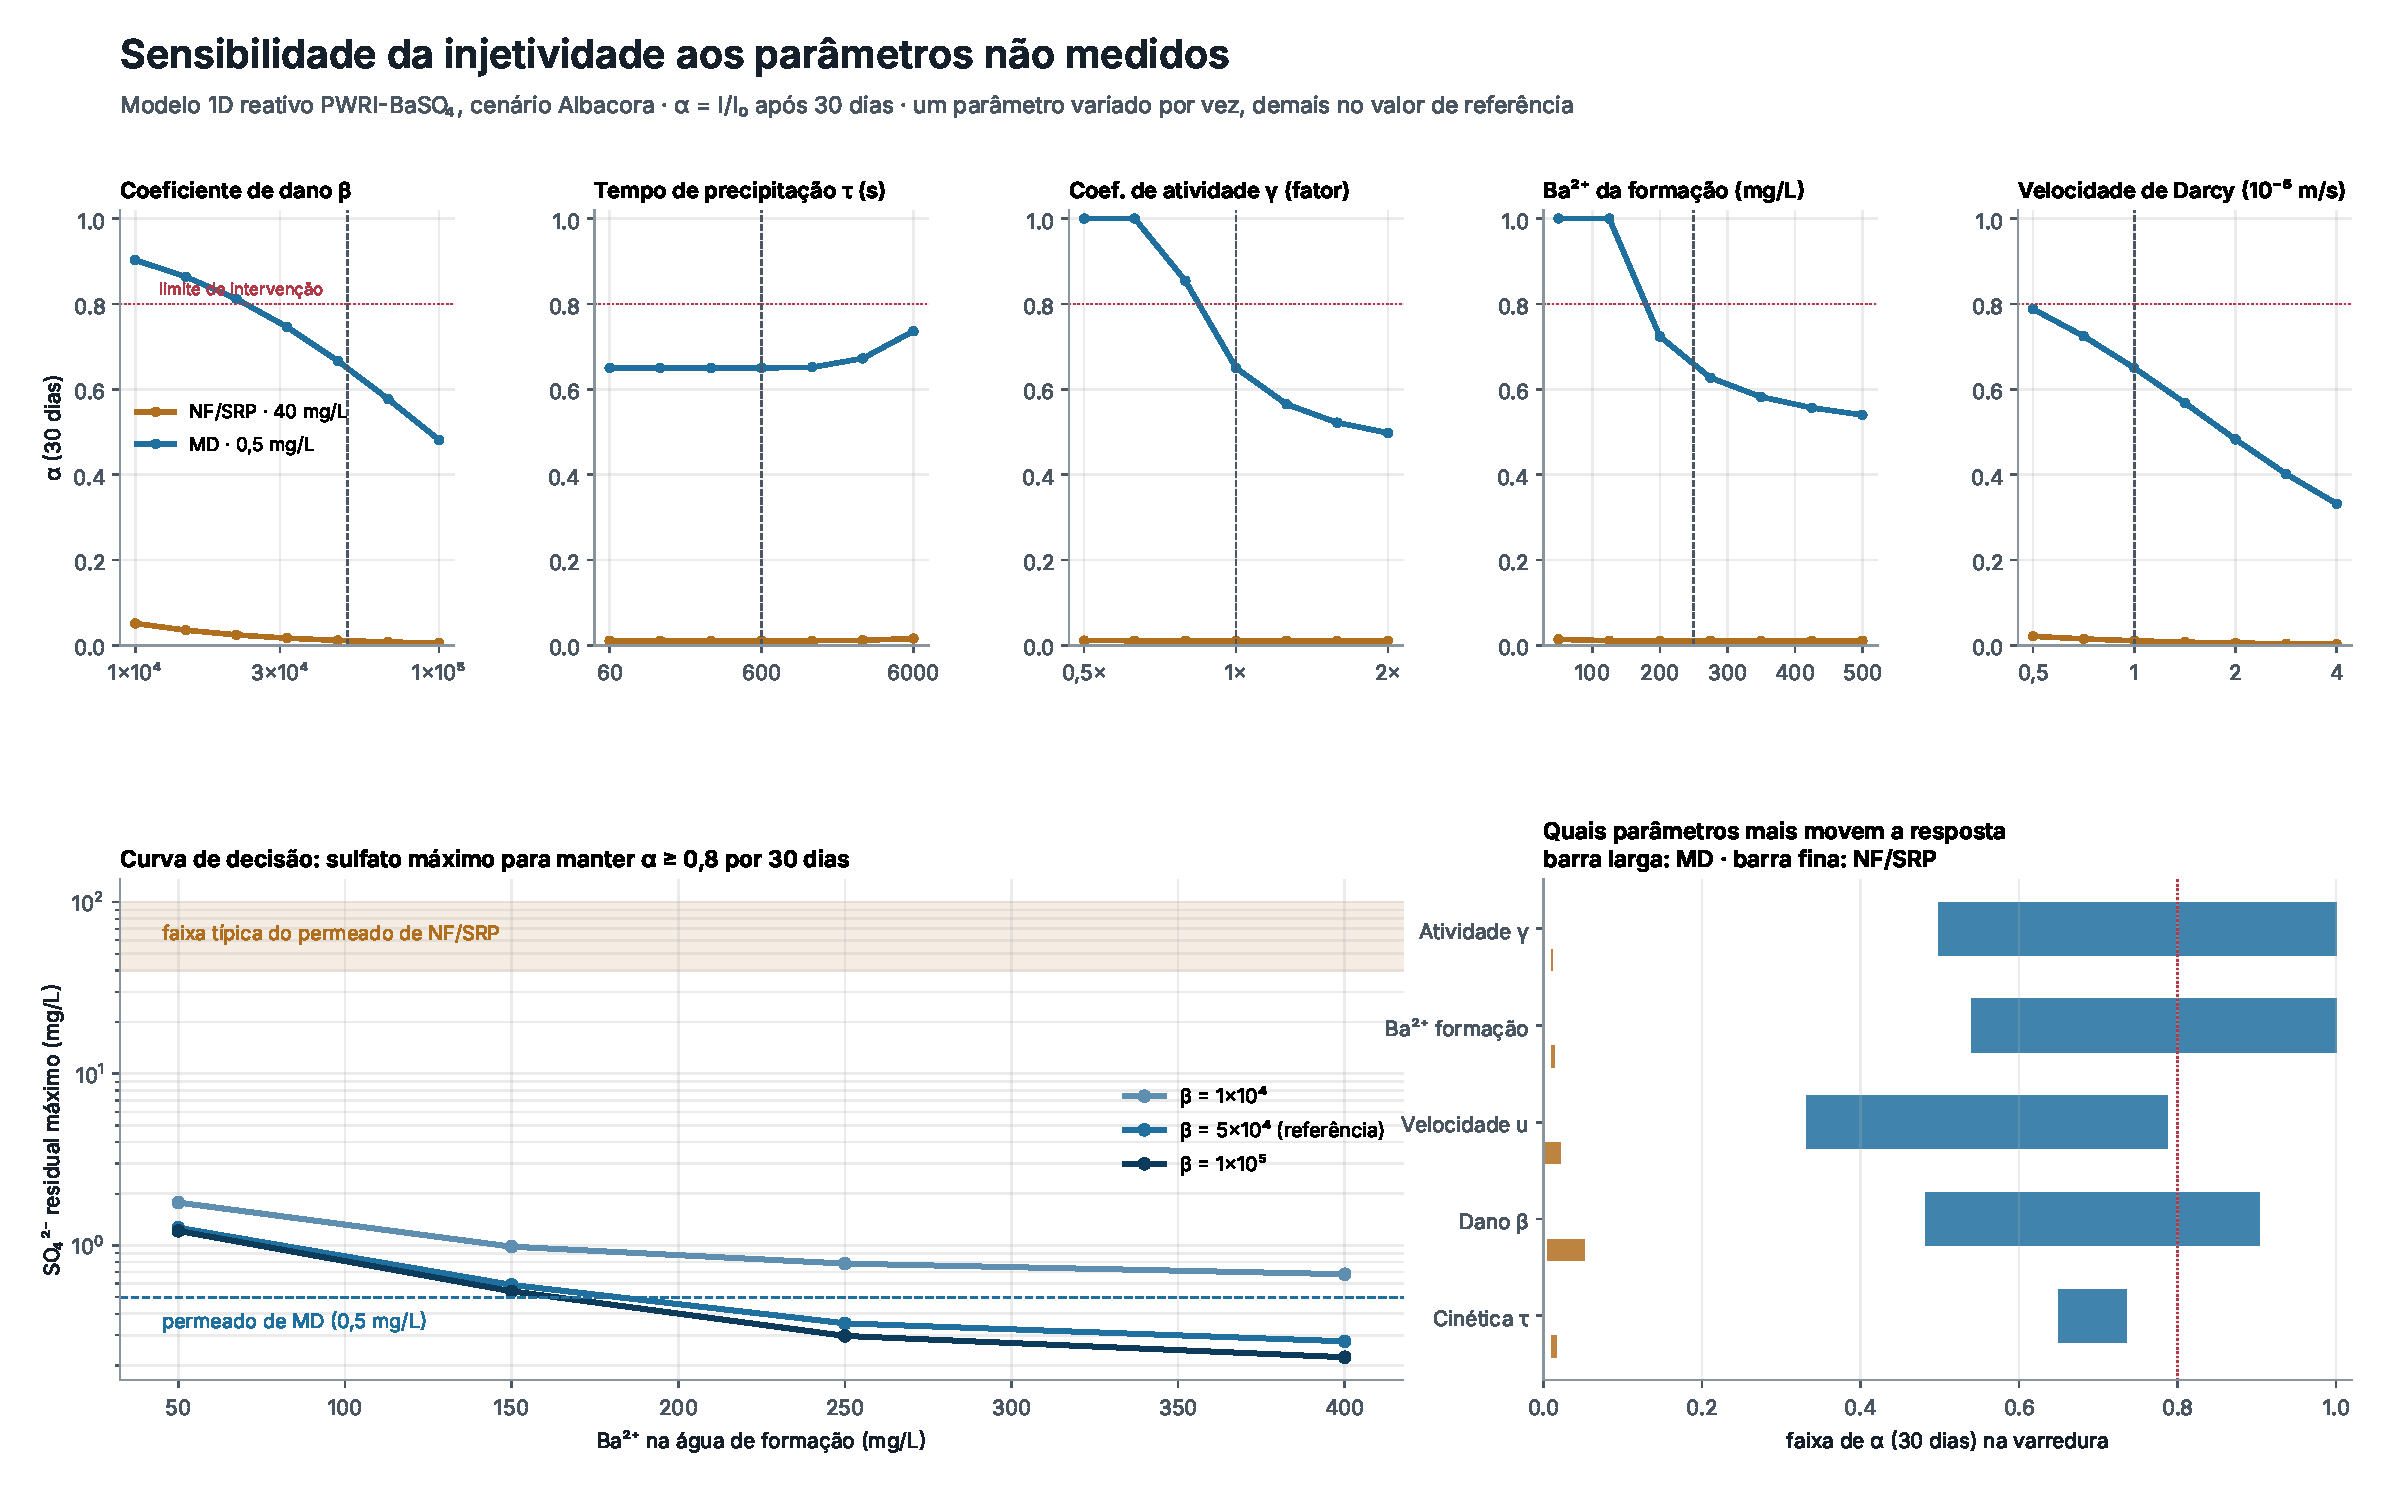
\includegraphics[width=0.77\textwidth]{sensibilidade_albacora.pdf}}{\fbox{\parbox{0.7\textwidth}{\centering Figura de sensibilidade: anexar sensibilidade\_albacora.pdf}}}
\caption{Sensibilidade de $\alpha$(30~d) aos parâmetros não medidos no modelo 1D reativo,
cenário Albacora. Acima: um parâmetro variado por vez, para nanofiltração (40~mg/L de
sulfato) e destilação por membrana (0,5~mg/L). Abaixo, à esquerda: sulfato residual
máximo para manter $\alpha \ge 0{,}8$ em 30 dias; à direita: faixa de $\alpha$ produzida por
cada parâmetro.}
\label{fig:sens}
\end{figure}

\subsection{Limitações e ligação com o projeto}
O estudo preliminar utiliza parâmetros assumidos e não constitui calibração de campo. Suas limitações definem o escopo do projeto:
\begin{itemize}
  \item geometria 1D, enquanto o entorno do poço é radial;
  \item cinética de primeira ordem, enquanto a cinética da barita pode apresentar dependência não linear da supersaturação \cite{nancollas1975};
  \item coeficientes de atividade fixos, em vez de um modelo de Pitzer \cite{pitzer1973};
  \item coeficiente de dano $\beta_{\mathrm{BaSO_4}}$ não calibrado experimentalmente;
  \item um único mecanismo (\ce{BaSO4}), sem \ce{SrSO4}, \ce{CaSO4}, \ce{CaCO3}, halita,
        finos e dano biológico;
  \item três cenários avaliados um a um, por simulação direta.
\end{itemize}
Os pontos anteriores serão investigados progressivamente pelo simulador (etapa 1) e pela identificação de
parâmetros com ensaios no LRAP+ (etapa 3), descritos na Seção~\ref{sec:metodo}. O último é a motivação central do projeto: com várias águas,
dezenas de íons e variáveis operacionais, o espaço de composições possíveis não pode ser
explorado cenário a cenário. É preciso um modelo substituto rápido e um método de
otimização que busque a composição ótima nesse espaço.

% ---------------------------------------------------------------------
\section{Questão científica, tecnológica ou de inovação e hipóteses}\itemedital{2.16 X}

\textbf{Questão:} é possível determinar, de forma adaptativa ao longo da vida do poço, as
condições ótimas da água de injeção (composição, nível de tratamento e vazão) que
preservam a injetividade, dadas as propriedades da rocha, as águas disponíveis (formação,
produzida e do mar) e as condições operacionais, mesmo quando parte dos parâmetros que
governam o dano não é medida diretamente?

\textbf{H0 (identificabilidade).} Os parâmetros do dano que não são medidos rotineiramente
(coeficientes de filtração e de dano, constantes cinéticas, salinidade e velocidade
críticas de desprendimento de finos) são identificáveis a partir de ensaios de
deslocamento com tomadas de pressão intermediárias, análise do efluente e microtomografia,
por meio de redes neurais informadas por física (PINN) em formulação inversa; o modelo
calibrado prevê ensaios não usados na calibração com erro inferior a 15\%.

\textbf{H1 (científica).} A injetividade de poços injetores pode resultar de mecanismos de dano
acoplados (incrustação, migração de finos, filtração, dano biológico), cuja resposta depende
conjuntamente da composição da água, das propriedades da rocha (mineralogia, teor de
argilas, estrutura porosa) e das condições operacionais (vazão, pressão e temperatura), e
é cumulativa ao longo do tempo. Consequentemente: (a) as condições ótimas da água não
podem ser definidas por limites independentes para cada parâmetro, como fazem os
critérios empíricos atuais; e (b) uma política de RL condicionada ao estado da rocha, da
operação e do dano acumulado preserva a injetividade de forma significativamente
superior à reotimização periódica míope, que escolhe a cada período a melhor condição
para o momento atual sem considerar suas consequências futuras.

\textit{Critérios de refutação:} (a) se condições definidas por limites independentes
atingirem desempenho equivalente ao da política, o acoplamento entre mecanismos não é
relevante na prática; (b) se a política não superar a reotimização míope em pelo menos
5\% nos cenários avaliados, a dependência da trajetória não é relevante, e a
otimização estática periódica é suficiente.

\textbf{H2 (validação experimental).} A política obtida no ambiente de simulação,
transposta para a escala de laboratório, preserva a injetividade medida em coreflood
melhor que as estratégias de referência, e o ambiente prevê a injetividade medida com erro
inferior a 15\%. \textit{Critério de refutação:} se a ordenação medida das sequências
diferir da prevista, ou o erro exceder 15\%, o ambiente não é confiável para decidir fora
da faixa em que foi calibrado.

As hipóteses são encadeadas: H0 fornece parâmetros calibrados e sua incerteza; H1 usa
esses parâmetros para testar o valor da decisão sequencial; H2 verifica em ensaios
se as decisões tomadas em simulação se sustentam no meio poroso real. Se H0 for apenas parcialmente confirmada, H1 continua
testável, com incerteza paramétrica maior incorporada ao treinamento do agente.

% ---------------------------------------------------------------------
\section{Objetivos}\itemedital{2.16 XI}

\subsection{Objetivo geral}
Desenvolver e validar uma metodologia que combine modelagem física do dano à formação,
identificação de parâmetros por redes neurais informadas por física e aprendizado por
reforço profundo para determinar dinamicamente as condições ótimas da água de injeção,
incluindo sua composição química e a vazão de injeção, de modo a mitigar a incrustação, a
migração de argilas e os demais mecanismos de dano que comprometem a injetividade, e validar
experimentalmente essas decisões em ensaios de coreflood. A ferramenta será estruturada de maneira modular, com interfaces para possível acoplamento futuro a modelos externos de recuperação de petróleo, de forma a incorporar objetivos produtivos específicos sem ampliar o escopo de validação do presente projeto.

\subsection{Objetivos específicos}
\begin{enumerate}[label=OE\arabic*.]
  \item Construir uma base de dados integrada de composição de águas, propriedades de
        rocha, variáveis operacionais e injetividade, a partir da literatura, de dados
        públicos de campo e dos ensaios do projeto.
  \item Estender o modelo físico do proponente para um simulador radial multiespécie do
        dano (incrustação, finos e argilas, filtração e reboco, dano biológico), capaz de
        separar o dano real da queda aparente por pressurização do reservatório.
  \item Realizar análise de sensibilidade global do simulador para identificar os
        parâmetros que mais afetam a injetividade e a decisão, e definir um conjunto
        mínimo de caracterização por rocha.
  \item Projetar e executar ensaios de deslocamento no LRAP+ e identificar os parâmetros
        não medidos por PINN em formulação inversa, com quantificação de incerteza e
        validação cega (teste da H0).
  \item Desenvolver um modelo substituto informado por física, parametrizado pelas
        propriedades da rocha, pelas condições operacionais e pelas ações, que sirva de
        ambiente rápido de treinamento.
  \item Treinar um agente de RL com restrições, robusto à incerteza paramétrica, que
        determine ao longo da vida do poço a composição, o tratamento (incluindo
        membranas de ePTFE/PTFE) e a vazão de injeção, e compará-lo com as referências
        definidas (teste da H1).
  \item Desenvolver um estimador do dano em operação, alimentado por dados de pressão e
        vazão de poços, e testá-lo com dados públicos de campo.
  \item Validar a política em ensaios de coreflood no LRAP+ e disponibilizar simulador,
        modelos e agentes como software aberto de apoio à decisão, com interface modular documentada para eventual integração futura de modelos externos de recuperação de petróleo (teste da H2 limitado à injetividade).
\end{enumerate}

% ---------------------------------------------------------------------
\section{Metodologia}\label{sec:metodo}\itemedital{2.16 XII}

A metodologia é organizada em sete etapas encadeadas: simulação física (1),
sensibilidade (2), calibração experimental por PINN inversa (3), modelo substituto (4),
treinamento e avaliação dos agentes acoplados ao ambiente de simulação (5), estimação com
dados de campo (6) e validação experimental da política com desenvolvimento do software
(7). O trabalho é computacional, exceto as duas campanhas de coreflood no LRAP+ (etapas 3
e 7). A
Figura~\ref{fig:infografico} resume os fatores considerados e sua relação com o ciclo de
decisão.

\begin{figure}[ht]
\centering
\IfFileExists{infografico_injetividade.pdf}{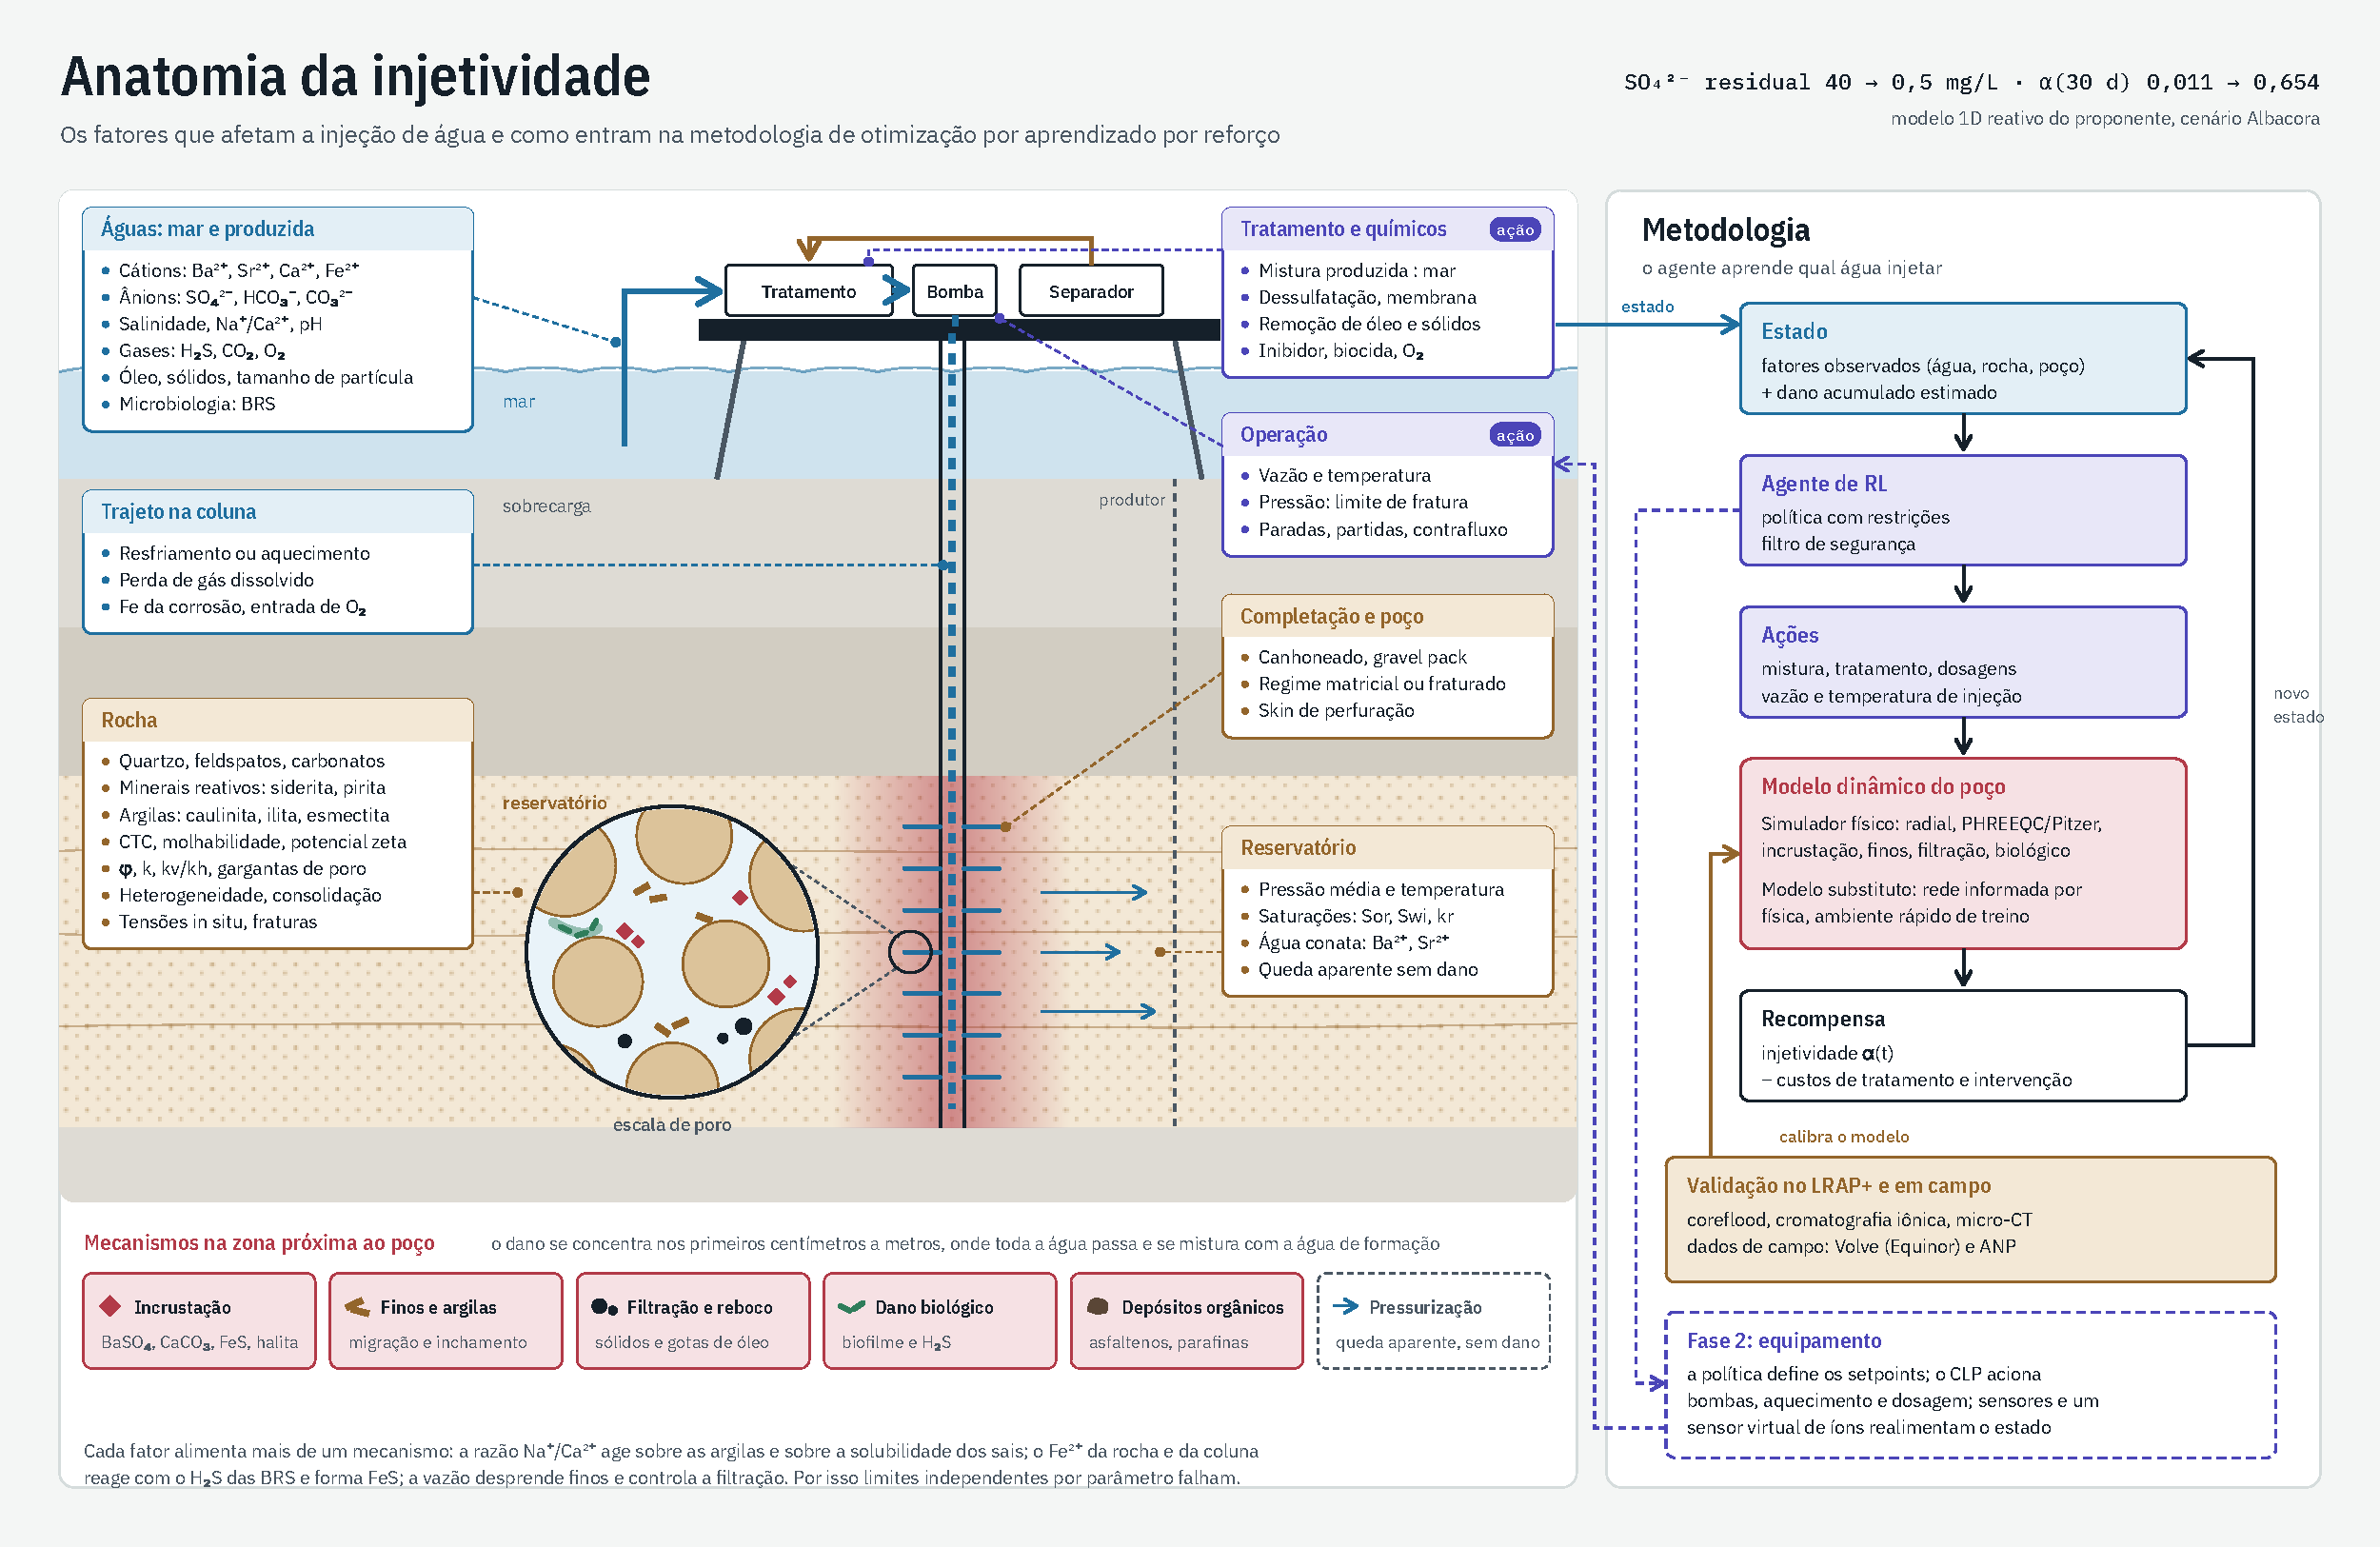
\includegraphics[width=0.74\textwidth]{infografico_injetividade.pdf}}{\fbox{\parbox{0.7\textwidth}{\centering Infográfico: anexar infografico\_injetividade.pdf}}}
\caption{Fatores que afetam a injetividade, desde as fontes de água até a escala de poro, e
sua relação com a metodologia: os fatores formam o estado do agente, as decisões sobre a
água formam as ações, o modelo dinâmico do poço calcula o dano e a injetividade retorna
como recompensa.}
\label{fig:infografico}
\end{figure}



\subsection{Formulação: decisão sequencial sob observação parcial}
A escolha da água é formulada como um processo de decisão de Markov parcialmente
observável. Em cada período $t$ (dias a semanas), o estado do sistema é
\begin{equation}
s_t = \left(\theta,\; w_t,\; o_t,\; d_t\right),
\end{equation}
em que $\theta$ reúne as propriedades da rocha e do poço (mineralogia, tipo e teor de
argilas, capacidade de troca catiônica, porosidade, permeabilidade, distribuição de
gargantas, completação) e os parâmetros do dano; $w_t$, a composição das águas disponíveis
(cátions, ânions, salinidade, pH, gases dissolvidos, óleo, sólidos e atividade
microbiológica); $o_t$, as condições operacionais (pressões de cabeça e de fundo,
temperatura, pressão média do reservatório); e $d_t$, o dano acumulado e sua distribuição
radial. Parte de $\theta$ e todo $d_t$ não são observados diretamente e são estimados (etapas
3 e 6).

A ação $a_t$ define as condições da água injetada: razão de mistura entre água produzida e
água do mar, grau de dessulfatação, tratamento por membrana, salinidade e razão
\ce{Na+}/\ce{Ca^2+}, remoção de óleo e sólidos, dosagens de inibidor, biocida e
sequestrante de oxigênio, vazão e temperatura de injeção. A recompensa combina a
manutenção da injetividade com os custos:
\begin{equation}
r_t = \alpha(t) - c_{\mathrm{trat}}(a_t) - c_{\mathrm{bomb}}(\Delta P_t) - c_{\mathrm{int}}\,\mathbb{1}[\alpha(t) < \alpha_{\min}],
\end{equation}
e o agente busca a política $\pi$ que maximiza o retorno esperado sob as restrições
$g_k(s_t,a_t)\le 0$:
\begin{equation}
\max_{\pi}\; \mathbb{E}_{\theta \sim p(\theta\mid\mathcal{D})}\;\mathbb{E}_{\pi}\!\left[\sum_{t=0}^{T} \gamma^{t} r_t\right]
\quad \text{s.a.} \quad g_k(s_t,a_t)\le 0 .
\end{equation}
As restrições $g_k$ incluem índices de saturação, salinidade e velocidade críticas para
estabilidade das argilas, pressão de fratura (manutenção do regime matricial), faixa de
vazão compatível com a reposição de volume do reservatório e limites do equipamento de
tratamento. A esperança sobre $p(\theta\mid\mathcal{D})$ incorpora a incerteza dos
parâmetros identificados na etapa 3. A vazão é variável de decisão do ponto de vista do
dano no entorno do poço; a vazão total do campo permanece como restrição externa. Nesta pesquisa, a recompensa se limita à preservação da injetividade e aos custos e restrições associados. Uma interface de acoplamento será definida para que, em aplicação futura, modelos de recuperação de petróleo de terceiros possam fornecer uma métrica adicional de desempenho ou uma restrição produtiva. Tal extensão exigirá modelos capazes de representar a influência da composição da água sobre a recuperação, compatibilidade entre as escalas temporais e validação própria; não integra o treinamento nem a avaliação experimental previstos neste projeto.

\subsection{Etapa 1 -- Modelo físico do dano}
O ponto de partida é o modelo 1D reativo da Seção~\ref{sec:prelim}, estendido para:
(i) geometria radial no entorno do poço, com completação canhoneada ou em poço aberto;
(ii) química multiespécie via PHREEQC com modelo de Pitzer (\ce{BaSO4}, \ce{SrSO4},
\ce{CaSO4}, \ce{CaCO3}, halita e \ce{FeS}), incluindo a variação de temperatura e
pressão ao longo da coluna e o aporte de ferro por corrosão; (iii) cinética de
precipitação de segunda ordem na supersaturação \cite{nancollas1975}, com tempo de
indução; (iv) migração e inchamento de argilas em função da salinidade, da composição
catiônica e da velocidade; (v) filtração profunda e reboco externo de sólidos e gotas,
dependentes da razão entre o tamanho das partículas e o das gargantas
\cite{pangsharma1997,bedrikovetsky2001}; (vi) módulo de dano biológico; e (vii) acoplamento
com um modelo simplificado de reservatório, para separar o dano no entorno do poço da
queda aparente de injetividade por aumento da pressão média e redução de mobilidade.
O simulador é verificado por balanço de massa e por reprodução de casos da literatura.

\subsection{Etapa 2 -- Análise de sensibilidade global}
Antes dos ensaios, o simulador é submetido a uma triagem de Morris \cite{morris1991}
seguida de índices de Sobol \cite{sobol2001} sobre os parâmetros não medidos e as
condições de rocha e operação. Além de $\alpha(t)$, são analisadas saídas relevantes para
a decisão: a ordenação de águas candidatas e as curvas de decisão (por exemplo, o
sulfato residual máximo para manter $\alpha \ge 0{,}8$). Os resultados definem quais
parâmetros precisam ser calibrados, quais podem ser fixados em valores de literatura,
qual o conjunto mínimo de caracterização por rocha e quais variáveis podem ser
retiradas do estado do agente. Um estudo preliminar desse tipo está na
Seção~\ref{sec:prelim}.

\subsection{Etapa 3 -- Ensaios no LRAP+ e identificação por PINN inversa}
\textbf{Desenho dos ensaios.} Antes de cada campanha, uma análise de identificabilidade
(perfis de verossimilhança sobre dados sintéticos do simulador) define quais medições
distinguem os parâmetros de interesse. Sabe-se, por exemplo, que a queda de pressão total
não separa o coeficiente de filtração do coeficiente de dano, o que exige tomadas de
pressão intermediárias \cite{bedrikovetsky2001}. Os ensaios serão realizados em plugs de
arenito de afloramento análogo e, quando disponíveis, de reservatório, caracterizados por
porosidade e permeabilidade (DV-4000), microtomografia e mineralogia (DRX e MEV, serviço
externo), com salmouras sintéticas de composição controlada. As campanhas isolam um
mecanismo por vez (compatibilidade e incrustação; redução escalonada de salinidade e
testes de vazão crítica para finos; injeção de suspensões calibradas para filtração) e
depois os combinam. Em cada ensaio são registrados vazão, diferencial de pressão total e,
quando o porta-testemunho permitir, em tomadas intermediárias, concentrações no efluente por
cromatografia de íons ao longo do tempo e microtomografia antes e depois, com
replicatas nas condições prioritárias. Esta é a primeira de duas campanhas: seus ensaios
são divididos em um conjunto de calibração e um de teste cego da H0; a segunda campanha é
dedicada à validação da política (etapa 7).

\textbf{PINN inversa.} Uma rede neural representa os campos de concentração, de depósito e
de pressão $\hat{u}(x,t)$ e é treinada para satisfazer simultaneamente os dados e as
equações do modelo \cite{raissi2019}:
\begin{equation}
\mathcal{L}(\phi_{\mathrm{NN}},\theta) =
\lambda_d\,\mathcal{L}_{\mathrm{dados}} + \lambda_r\,\mathcal{L}_{\mathrm{EDP}} + \lambda_b\,\mathcal{L}_{\mathrm{contorno}},
\end{equation}
em que os parâmetros desconhecidos $\theta$ (coeficientes de filtração e de dano,
constantes cinéticas, salinidade e velocidade críticas) são variáveis treináveis. Onde a
forma da lei constitutiva é incerta, como $k(\sigma)$, uma pequena rede aprende a própria
relação. A incerteza é estimada por conjuntos de redes ou formulação bayesiana, resultando
em $p(\theta\mid\mathcal{D})$. Como PINNs têm dificuldade com frentes abruptas em
transporte em meios porosos \cite{fuks2020}, serão usadas ponderação adaptativa das
perdas, treinamento progressivo no tempo e difusão artificial controlada, e os resultados
serão comparados com a calibração clássica por mínimos quadrados sobre o simulador de
volumes finitos.

\textbf{Validação cega (H0).} Os ensaios são divididos em um conjunto de calibração e um
conjunto de teste, com composições e vazões diferentes. O modelo calibrado prevê o
conjunto de teste sem novo ajuste, e compara-se a injetividade, o perfil de depósito na
microtomografia e a composição do efluente.

\subsection{Etapa 4 -- Modelo substituto}
O agente exige milhares de episódios, o que torna inviável usar o simulador completo como
ambiente. Será treinado um operador neural (DeepONet ou FNO) \cite{lu2021deeponet,li2021fno},
com resíduo físico na função de perda, que recebe $\theta$, o estado e a sequência de
ações e devolve a evolução do dano e de $\alpha(t)$. Os dados de treino são gerados pelo
simulador, com amostragem por hipercubo latino sobre $p(\theta\mid\mathcal{D})$ e sobre o
espaço de operação. A validação usa simulações não vistas, com metas de $R^2$, erro em
$\alpha$ e ganho de tempo de avaliação, e a incerteza do substituto é estimada por
conjunto de redes, para que o agente evite regiões em que o substituto não é confiável.

\subsection{Etapa 5 -- Agente de aprendizado por reforço}
O agente é treinado sobre o substituto, com verificação periódica no simulador completo.
Como nenhum algoritmo é superior em todos os problemas, serão avaliadas as oito famílias de
aprendizado por reforço, cada uma com um papel definido no projeto
(Tabela~\ref{tab:rl}).

\begin{table}[!htbp]
\centering
\footnotesize
\setstretch{1.0}
\caption{Famílias de algoritmos de RL avaliadas, seu uso no projeto e aplicações de referência.}
\label{tab:rl}
\begin{tabularx}{\textwidth}{@{}>{\raggedright\arraybackslash}p{0.22\textwidth}>{\raggedright\arraybackslash}X>{\raggedright\arraybackslash}p{0.14\textwidth}@{}}
\toprule
\textbf{Família e algoritmos} & \textbf{Uso no projeto} & \textbf{Aplicações} \\
\midrule
\textbf{Tabulares:} iteração de política e de valor, Monte Carlo, TD(0), TD($\lambda$), SARSA, Q-learning
 & Versão discretizada e reduzida do problema (poucas águas candidatas, estados agregados). A iteração de valor fornece o ótimo exato dessa versão, usado como gabarito para verificar os métodos profundos.
 & \cite{lutter2021rvi,mcuav2022,rizvi2021tnnls,rizvi2023jas} \\
\addlinespace
\textbf{Valor com redes neurais:} DQN, Double DQN, C51, QR-DQN, Rainbow
 & Ações discretas (catálogo de águas e de níveis de tratamento). As versões distribucionais (C51, QR-DQN) estimam a distribuição do retorno e permitem políticas sensíveis a risco, avaliadas pelo CVaR.
 & \cite{fang2022hvac,alsayed2026,iccc2024nav} \\
\addlinespace
\textbf{Gradiente de política:} REINFORCE, gradiente natural, TRPO
 & Referências de base para ações contínuas; o TRPO fundamenta a otimização com restrições por região de confiança (CPO) \cite{achiam2017}.
 & \cite{nakamura2005,centurelli2022} \\
\addlinespace
\textbf{Ator-crítico:} A2C, A3C, DDPG, TD3, SAC, PPO
 & Candidatos principais para ações contínuas (proporções de mistura, dosagens, vazão), em versões com restrições por multiplicadores de Lagrange \cite{ray2019}.
 & \cite{jobe2025hvac,zhong2022designs,du2021hvac,fan2024uuv,benhazem2026,silvestri2024,wang2025dce,elagroudi2025} \\
\addlinespace
\textbf{Baseados em modelo:} Dyna-Q, PILCO, PETS, MBPO, Dreamer, MuZero
 & Usam o substituto para gerar transições e reduzir chamadas ao simulador. PILCO e PETS são eficientes quando cada amostra é cara, como no ajuste ao ambiente em escala de laboratório (etapa 7); o Dreamer, com modelo latente, trata a observação parcial.
 & \cite{hu2019sym,ifac2025pilco,ye2025mbrl,wu2023daydreamer} \\
\addlinespace
\textbf{Multiagente:} Q-learning independente, MADDPG, VDN, QMIX, MAPPO
 & Dois usos: vários poços injetores que compartilham a capacidade de tratamento; e um agente por variável de tratamento (mistura, dessulfatação, dosagens), coordenados.
 & \cite{harrold2022,yun2025ro,dcmg2025,qiu2023} \\
\addlinespace
\textbf{Offline:} BCQ, CQL, IQL, AWAC, TD3+BC
 & Aprendizado a partir de históricos de operação já registrados, sem experimentação no poço; política inicial conservadora.
 & \cite{he2025disaiql,nair2020awac} \\
\addlinespace
\textbf{Hierárquicos:} opções, MAXQ, HIRO
 & Correspondem à hierarquia do problema: o nível alto escolhe a água (dias a semanas) e o nível baixo ajusta vazão e dosagens dentro de cada período.
 & \cite{yang2022hrl,engappai2023hrl,wan2025hrl,nachum2018hiro} \\
\bottomrule
\end{tabularx}
\end{table}

A avaliação é feita em dois estágios, para que a comparação ampla caiba no orçamento
computacional:
\begin{enumerate}[label=(\alph*)]
  \item \textit{Triagem:} um ou dois representantes de cada família são treinados em um
        ambiente reduzido (horizonte curto, menos cenários, três sementes). Na versão
        discretizada, o desempenho é normalizado pelo ótimo exato da iteração de valor. Os
        critérios para avançar são o retorno normalizado, a taxa de violação de
        restrições, a eficiência amostral (retorno por chamada ao simulador) e o custo
        computacional.
  \item \textit{Aprofundamento:} os três ou quatro melhores da triagem, mais o PPO com
        restrições como referência fixa, seguem para o protocolo estatístico completo da
        Seção~\ref{sec:incerteza}.
\end{enumerate}
Os métodos multiagente e hierárquicos são avaliados nos cenários em que se aplicam (vários
poços e várias variáveis de tratamento), e os métodos \textit{offline} são avaliados por avaliação
fora da política sobre históricos simulados e públicos. Cada algoritmo é testado com
observação completa e em versão recorrente (LSTM), e os hiperparâmetros são ajustados com o
mesmo orçamento para todos, usando bibliotecas de referência (Stable-Baselines3, OmniSafe e
d3rlpy). A
robustez à incerteza é obtida sorteando $\theta \sim p(\theta\mid\mathcal{D})$ a cada
episódio, de modo que a política funcione em toda a faixa plausível dos parâmetros, e não
apenas no valor médio \cite{nasir2022}. A observação parcial é tratada fornecendo à
política a estimativa do estado latente produzida pelo estimador da etapa 6, ou por meio
de uma política recorrente. Um filtro de segurança projeta as ações propostas na região
viável definida pelas restrições $g_k$. O tratamento por membranas de ePTFE/PTFE entra
como ação, com custo energético associado ao aproveitamento de calor residual.

Para testar a H1, a política é comparada, nos mesmos cenários de rocha, água e operação,
com três referências: (i) os critérios empíricos atuais, baseados em limites
independentes por parâmetro; (ii) a melhor condição fixa para todo o horizonte, obtida por
otimização bayesiana; e (iii) a reotimização periódica míope, em que a otimização
bayesiana é reaplicada a cada período com as condições do momento. A referência (iii) é a
principal, pois isola o ganho atribuível à antecipação das consequências futuras. As
métricas são a injetividade média e final no horizonte, o custo total, o número de
violações de restrição e a ordenação das alternativas. O protocolo estatístico de
comparação está na Seção~\ref{sec:incerteza}.

\subsection{Quantificação de incerteza e critérios estatísticos}\label{sec:incerteza}

\textbf{Incerteza dos parâmetros identificados pela PINN (H0).} A incerteza de cada
parâmetro $\theta_j$ será avaliada segundo o Guia para a Expressão da Incerteza de Medição
(GUM) \cite{gum2008} e seu Suplemento 1 \cite{gums12008}, com as componentes:

\begin{center}
\small
\begin{tabularx}{\textwidth}{@{}l>{\raggedright\arraybackslash}X>{\raggedright\arraybackslash}X@{}}
\toprule
\textbf{Componente} & \textbf{Fonte} & \textbf{Avaliação} \\
\midrule
Tipo A, repetibilidade & Variação entre replicatas de coreflood nas mesmas condições & $u_A = s/\sqrt{n}$ a partir das estimativas de $\theta_j$ em cada replicata \\
Tipo A, estimação & Variabilidade do próprio estimador (inicialização e dados) & Conjunto de PINNs treinadas com sementes diferentes \cite{lakshminarayanan2017} e \textit{bootstrap} dos resíduos \cite{efron1993} \\
Tipo B, instrumentos & Transdutores de pressão, bomba, cromatografia iônica, temperatura, dimensões e porosidade do plug & Certificados de calibração e especificações, com distribuições normal ou retangular \\
Tipo B, modelo & Escolha da lei constitutiva (aditiva, porosidade crítica, aprendida) & Dispersão entre as estimativas obtidas com leis alternativas \\
\bottomrule
\end{tabularx}
\end{center}

\noindent Os coeficientes de sensibilidade $c_i = \partial\theta_j/\partial x_i$ às grandezas de
entrada são obtidos por diferenciação automática da própria PINN, e a incerteza padrão
combinada é
\begin{equation}
u_c(\theta_j) = \sqrt{u_{A}^{2} + \sum_i c_i^{2}\,u_{B,i}^{2} + u_{\mathrm{mod}}^{2} + 2\sum_{i<k} c_i c_k\, u(x_i,x_k)},
\end{equation}
com graus de liberdade efetivos pela fórmula de Welch-Satterthwaite e incerteza expandida
$U = k\,u_c$, com $k$ da distribuição $t$ para 95\% de abrangência. Como o modelo é não
linear, o resultado linearizado será confrontado com a propagação por Monte Carlo do
Suplemento 1: as grandezas de entrada são sorteadas de suas distribuições, a
identificação é repetida (sobre o substituto, para viabilizar $10^4$ a $10^5$ amostras) e
obtém-se a distribuição de $\theta_j$, seu intervalo de abrangência de 95\% e a matriz de
covariância entre parâmetros, que evidencia correlações como a entre os coeficientes de
filtração e de dano. Parâmetros estritamente positivos serão testados quanto à aderência a
distribuições normal e log-normal (Shapiro-Wilk e Anderson-Darling), e a formulação
bayesiana da PINN \cite{yang2021bpinn} será usada como verificação independente da
distribuição \textit{a posteriori}. A identificabilidade é verificada por perfis de
verossimilhança \cite{raue2009}.

\textbf{Demonstração estatística da H0.} Três testes, em sequência:
\begin{enumerate}[label=(\roman*)]
  \item \textit{Recuperação em dados sintéticos:} cerca de 200 conjuntos gerados pelo simulador
        com $\theta$ conhecido e ruído compatível com as incertezas tipo A e tipo B; o
        método deve ser não enviesado (teste $t$ sobre o erro) e seus intervalos de 95\% devem
        conter o valor verdadeiro em proporção compatível com 95\% (teste binomial).
  \item \textit{Concordância com a calibração clássica:} as estimativas da PINN e do ajuste por
        mínimos quadrados sobre o simulador de volumes finitos devem ser compatíveis dentro
        das incertezas expandidas.
  \item \textit{Previsão cega:} para cada ensaio de teste, o erro normalizado
        $E_n = |y_{\mathrm{prev}} - y_{\mathrm{med}}| \big/ \sqrt{U_{\mathrm{prev}}^2 + U_{\mathrm{med}}^2}$
        deve satisfazer $E_n \le 1$ \cite{iso13528}, e a calibração das incertezas
        previstas é verificada pela cobertura empírica dos intervalos e pelo histograma da
        transformada integral de probabilidade.
\end{enumerate}

\textbf{Comparação entre algoritmos de RL e teste da H1.} O desempenho de algoritmos de RL
varia muito entre sementes aleatórias \cite{henderson2018}. Cada algoritmo será treinado
com pelo menos 10 sementes e avaliado em um conjunto de cenários de teste não
usados no treino, com $\theta$ sorteado por Monte Carlo de $p(\theta\mid\mathcal{D})$. A
incerteza paramétrica é propagada à decisão: para cada política, obtém-se a distribuição
de $\alpha(T)$ e do custo, reportando mediana, quantis P10 e P90 e o valor em risco
condicional (CVaR) dos 10\% piores cenários. A agregação segue as recomendações de Agarwal
et al. \cite{agarwal2021}: média interquartil (IQM) do retorno normalizado, intervalos de
confiança de 95\% por \textit{bootstrap} estratificado sobre sementes e cenários, perfis
de desempenho e probabilidade de melhoria entre pares de algoritmos. Comparações pareadas
(mesmos cenários) usam o teste de postos sinalizados de Wilcoxon com correção de Holm para
múltiplas comparações. O algoritmo escolhido é o de maior IQM cujo intervalo de confiança
não se sobreponha ao dos demais, ou, havendo sobreposição, o de menor taxa de violação de
restrições e menor CVaR. A H1 é considerada confirmada se a probabilidade de melhoria da
política sobre a reotimização míope tiver intervalo de 95\% acima de 0,5 e o ganho mediano
superar 5\%.

\subsection{Etapa 6 -- Estimação em operação e validação com dados de campo}
A mesma formulação inversa da etapa 3 é aplicada a dados de poço para estimar a evolução
do dano e ajustar os parâmetros de cada poço. A separação entre dano e pressurização usa
os dados de pressão de fundo e vazão, com análise do gráfico de Hall e de períodos de
fechamento. O estimador é testado com os dados diários públicos do campo de Volve
(Equinor), que incluem pressão de fundo, pressão de cabeça e volumes injetados, e as
séries de injeção da ANP são usadas para testar a generalização do substituto a
históricos de longo prazo. A incerteza do estimador permite ainda avaliar o valor da
informação, isto é, quando vale a pena coletar uma nova medição antes de mudar a água.

\subsection{Etapa 7 -- Validação experimental da política e software}
O teste final é experimental e verifica se as decisões tomadas no ambiente de simulação se
sustentam no meio poroso real. Como o horizonte de vida do poço não cabe em um ensaio, a
política é avaliada em escala de laboratório: o ambiente de simulação é reconfigurado com a
geometria linear, as dimensões dos plugs e a faixa de vazões do coreflood, calibrado com
os dados da primeira campanha, e o agente é ajustado nesse ambiente. Na segunda campanha
no LRAP+, plugs da mesma rocha recebem, com o mesmo volume injetado e em réplicas, três
sequências de águas e vazões: (i) a recomendada pela política de RL; (ii) a da
reotimização periódica míope; e (iii) a do critério empírico de limites independentes por
parâmetro. As sequências e as previsões do ambiente são definidas e registradas antes dos
ensaios, para que a comparação seja cega em relação aos resultados. Medem-se $\alpha(t)$,
os perfis de pressão, a composição do efluente e o depósito por microtomografia.

Dois resultados são extraídos. O primeiro é a ordenação medida das três sequências, que
testa experimentalmente a H1 nas condições ensaiadas. O segundo é o erro entre a
injetividade prevista pelo ambiente de simulação e a medida (teste da H2), avaliado com as
incertezas expandidas da medição e da previsão pelo erro normalizado $E_n$
(Seção~\ref{sec:incerteza}).

O resultado tecnológico é um pacote de software aberto que integra o simulador físico, o
modelo substituto, a PINN inversa, o ambiente de treinamento no padrão Gymnasium, os
agentes treinados e o protocolo estatístico de avaliação, com uma interface de apoio à
decisão que recebe os dados de água, rocha e operação de um poço e devolve a composição, o
tratamento e a vazão recomendados, com a incerteza associada. A arquitetura separará o módulo de avaliação do dano e da injetividade do módulo de decisão e especificará uma interface externa de troca de dados. Essa interface documentará entradas de composição química, condições de injeção e estado do reservatório, bem como saídas esperadas de desempenho de recuperação e restrições operacionais. Em eventual aplicação industrial, um modelo externo capaz de responder a alterações na composição da água poderá ser conectado à otimização para formular objetivos múltiplos ou restrições de recuperação. A especificação dessa interface será entregue no software; o acoplamento efetivo com simuladores proprietários, a otimização de EOR e sua validação não integram as metas deste projeto. O desenvolvimento segue
práticas de engenharia de software (controle de versão, testes automatizados, integração
contínua e documentação), para que o ambiente possa ser reutilizado por outros grupos e
pela indústria.

% ---------------------------------------------------------------------
\section{Metas, entregas verificáveis e indicadores de acompanhamento}\itemedital{2.16 XIII, XVI; 6.3.4}

\subsection{Metas e entregas verificáveis}\itemedital{2.16 XIII}

{\small\setstretch{1.0}
\begin{longtable}{@{}p{0.05\textwidth}>{\raggedright\arraybackslash}p{0.43\textwidth}>{\raggedright\arraybackslash}p{0.37\textwidth}>{\centering\arraybackslash}p{0.07\textwidth}@{}}
\toprule
\textbf{\#} & \textbf{Meta / entrega} & \textbf{Indicador} & \textbf{Mês} \\
\midrule
\endhead
M1 & Base de dados integrada (águas, rocha, operação, injetividade) & $\geq$ 300 registros com metadados completos; documentação pública & 9 \\
M2 & Simulador radial multiespécie & Balanço de massa fechado em $\geq$ 99\%; reprodução de casos da literatura & 15 \\
M3 & Análise de sensibilidade global & Índices de Sobol para todos os parâmetros não medidos; conjunto mínimo de caracterização definido & 18 \\
M4 & Parâmetros identificados por PINN inversa (teste da H0) & 1 campanha de coreflood com replicatas (calibração e teste cego); erro na previsão cega de $\alpha$ $\leq$ 15\%; fechamento do balanço iônico $\geq$ 90\% & 24 \\
M5 & Modelo substituto validado & $R^2 \geq$ 0,95 em teste cego; avaliação $\geq 10^3\times$ mais rápida que o simulador & 26 \\
M6 & Agente de RL robusto e comparado com as três referências (teste da H1) & Ganho sobre a reotimização míope $\geq$ 5\% em $\geq$ 50 cenários de teste; correlação de Spearman da ordenação $\geq$ 0,8 & 34 \\
M7 & Estimador do dano em operação & Separação entre dano e pressurização em dados de Volve; erro de previsão em janela futura $\leq$ 10\% & 38 \\
M8 & Validação da política em coreflood (teste da H2) & Sequência do agente com $\alpha$ final superior às de referência, em réplicas; erro do ambiente de simulação $\leq$ 15\% & 44 \\
M9 & Ferramenta de apoio à decisão (código aberto) & Repositório versionado (código, dados e modelos) & 46 \\
M10 & Produção científica (Seção~\ref{sec:resultados}) & 3 artigos submetidos a periódicos A1/A2 (P1--P3); 2 trabalhos completos apresentados no Rio Oil \& Gas (C1) e em evento da SPE (C2) & 20--46 \\
\bottomrule
\end{longtable}
}

\subsection{Indicadores de acompanhamento}\itemedital{2.16 XVI}
O acompanhamento acompanha os quatro relatórios parciais que condicionam a liberação das
parcelas (item 8.4). Em cada relatório são verificadas as metas previstas para o período e
indicadores de processo que mostram o avanço das atividades em curso, mesmo antes de a meta
correspondente ser concluída.

{\small\setstretch{1.0}
\begin{longtable}{@{}>{\raggedright\arraybackslash}p{0.11\textwidth}>{\raggedright\arraybackslash}p{0.26\textwidth}>{\raggedright\arraybackslash}p{0.57\textwidth}@{}}
\toprule
\textbf{Relatório} & \textbf{Metas a comprovar} & \textbf{Indicadores de processo} \\
\midrule
\endhead
R1 (mês 12) & M1 & Revisão sistemática concluída; simulador radial com módulo de incrustação implementado e balanço de massa verificado; plano experimental da campanha 1 definido pela análise de identificabilidade e ensaios iniciados; doutorando matriculado e iniciação científica selecionada; credenciamento no PEM; 2 ações em escolas \\
R2 (mês 24) & M2, M3, M4 & Número de corefloods da campanha 1 realizados com réplicas e dados depositados no Zenodo; erro da previsão cega da H0; primeira versão do modelo substituto; trabalho C1 apresentado; disciplina eletiva ofertada; ações de divulgação acumuladas \\
R3 (mês 36) & M5, M6 & Número de algoritmos triados e aprofundados; resultado estatístico da H1 (IQM, probabilidade de melhoria); P1 e P2 submetidos; estimador aplicado aos dados de Volve; sequências e previsões da campanha 2 registradas antes dos ensaios; exame de qualificação do doutorando; primeira proposta a edital externo submetida \\
RF (mês 48) & M7, M8, M9, M10 & Resultado da campanha 2 (teste da H2); C2 apresentado e P3 submetido; software público com identificador permanente; tese em fase final; indicadores consolidados de divulgação (escolas, participantes, vídeos, acessos ao simulador) \\
\bottomrule
\end{longtable}
}

\noindent Em todos os relatórios são informados também a execução orçamentária por
elemento de despesa e o percentual de atividades do cronograma cumpridas no prazo.

% ---------------------------------------------------------------------
\section{Cronograma físico em meses corridos}\itemedital{2.16 XIV; Anexo 1 II.II-g}
O cronograma é contado a partir do início da execução; os relatórios parciais condicionam o desembolso de parcelas, conforme item 8.4. O detalhamento mensal será espelhado no plano de trabalho do SisFAPERJ.
A Figura~\ref{fig:gantt} apresenta as atividades mês a mês, com as metas (M), as publicações (C, P) e os relatórios parciais que condicionam as parcelas (R).

\begin{figure}[!htbp]
\begin{tikzpicture}[x=0.255cm,y=0.42cm,font=\scriptsize]
\fill[gray!18] (0,1.25) rectangle (12,2.1);
\node at (6,1.68) {\textbf{Ano 1}};
\fill[gray!10] (12,1.25) rectangle (24,2.1);
\node at (18,1.68) {\textbf{Ano 2}};
\fill[gray!18] (24,1.25) rectangle (36,2.1);
\node at (30,1.68) {\textbf{Ano 3}};
\fill[gray!10] (36,1.25) rectangle (48,2.1);
\node at (42,1.68) {\textbf{Ano 4}};
\node[font=\tiny] at (0.5,0.7) {1};
\node[font=\tiny] at (2.5,0.7) {3};
\node[font=\tiny] at (5.5,0.7) {6};
\node[font=\tiny] at (8.5,0.7) {9};
\node[font=\tiny] at (11.5,0.7) {12};
\node[font=\tiny] at (14.5,0.7) {15};
\node[font=\tiny] at (17.5,0.7) {18};
\node[font=\tiny] at (20.5,0.7) {21};
\node[font=\tiny] at (23.5,0.7) {24};
\node[font=\tiny] at (26.5,0.7) {27};
\node[font=\tiny] at (29.5,0.7) {30};
\node[font=\tiny] at (32.5,0.7) {33};
\node[font=\tiny] at (35.5,0.7) {36};
\node[font=\tiny] at (38.5,0.7) {39};
\node[font=\tiny] at (41.5,0.7) {42};
\node[font=\tiny] at (44.5,0.7) {45};
\node[font=\tiny] at (47.5,0.7) {48};
\draw[gray!60,line width=0.5pt] (0,0.35) -- (0,-14);
\draw[gray!12,line width=0.3pt] (1,0.35) -- (1,-14);
\draw[gray!12,line width=0.3pt] (2,0.35) -- (2,-14);
\draw[gray!12,line width=0.3pt] (3,0.35) -- (3,-14);
\draw[gray!12,line width=0.3pt] (4,0.35) -- (4,-14);
\draw[gray!12,line width=0.3pt] (5,0.35) -- (5,-14);
\draw[gray!30,line width=0.3pt] (6,0.35) -- (6,-14);
\draw[gray!12,line width=0.3pt] (7,0.35) -- (7,-14);
\draw[gray!12,line width=0.3pt] (8,0.35) -- (8,-14);
\draw[gray!12,line width=0.3pt] (9,0.35) -- (9,-14);
\draw[gray!12,line width=0.3pt] (10,0.35) -- (10,-14);
\draw[gray!12,line width=0.3pt] (11,0.35) -- (11,-14);
\draw[gray!60,line width=0.5pt] (12,0.35) -- (12,-14);
\draw[gray!12,line width=0.3pt] (13,0.35) -- (13,-14);
\draw[gray!12,line width=0.3pt] (14,0.35) -- (14,-14);
\draw[gray!12,line width=0.3pt] (15,0.35) -- (15,-14);
\draw[gray!12,line width=0.3pt] (16,0.35) -- (16,-14);
\draw[gray!12,line width=0.3pt] (17,0.35) -- (17,-14);
\draw[gray!30,line width=0.3pt] (18,0.35) -- (18,-14);
\draw[gray!12,line width=0.3pt] (19,0.35) -- (19,-14);
\draw[gray!12,line width=0.3pt] (20,0.35) -- (20,-14);
\draw[gray!12,line width=0.3pt] (21,0.35) -- (21,-14);
\draw[gray!12,line width=0.3pt] (22,0.35) -- (22,-14);
\draw[gray!12,line width=0.3pt] (23,0.35) -- (23,-14);
\draw[gray!60,line width=0.5pt] (24,0.35) -- (24,-14);
\draw[gray!12,line width=0.3pt] (25,0.35) -- (25,-14);
\draw[gray!12,line width=0.3pt] (26,0.35) -- (26,-14);
\draw[gray!12,line width=0.3pt] (27,0.35) -- (27,-14);
\draw[gray!12,line width=0.3pt] (28,0.35) -- (28,-14);
\draw[gray!12,line width=0.3pt] (29,0.35) -- (29,-14);
\draw[gray!30,line width=0.3pt] (30,0.35) -- (30,-14);
\draw[gray!12,line width=0.3pt] (31,0.35) -- (31,-14);
\draw[gray!12,line width=0.3pt] (32,0.35) -- (32,-14);
\draw[gray!12,line width=0.3pt] (33,0.35) -- (33,-14);
\draw[gray!12,line width=0.3pt] (34,0.35) -- (34,-14);
\draw[gray!12,line width=0.3pt] (35,0.35) -- (35,-14);
\draw[gray!60,line width=0.5pt] (36,0.35) -- (36,-14);
\draw[gray!12,line width=0.3pt] (37,0.35) -- (37,-14);
\draw[gray!12,line width=0.3pt] (38,0.35) -- (38,-14);
\draw[gray!12,line width=0.3pt] (39,0.35) -- (39,-14);
\draw[gray!12,line width=0.3pt] (40,0.35) -- (40,-14);
\draw[gray!12,line width=0.3pt] (41,0.35) -- (41,-14);
\draw[gray!30,line width=0.3pt] (42,0.35) -- (42,-14);
\draw[gray!12,line width=0.3pt] (43,0.35) -- (43,-14);
\draw[gray!12,line width=0.3pt] (44,0.35) -- (44,-14);
\draw[gray!12,line width=0.3pt] (45,0.35) -- (45,-14);
\draw[gray!12,line width=0.3pt] (46,0.35) -- (46,-14);
\draw[gray!12,line width=0.3pt] (47,0.35) -- (47,-14);
\draw[gray!60,line width=0.5pt] (48,0.35) -- (48,-14);
\fill[gray!6] (-15.6,-1) rectangle (48,0);
\node[anchor=west] at (-15.4,-0.5) {A1 Revisão e banco de dados};
\fill[blue!55!black] (0,-0.78) rectangle (9,-0.22);
\node[anchor=west] at (-15.4,-1.5) {A2 Simulador físico radial};
\fill[blue!55!black] (0,-1.78) rectangle (15,-1.22);
\fill[gray!6] (-15.6,-3) rectangle (48,-2);
\node[anchor=west] at (-15.4,-2.5) {A3 Sensibilidade e identificab.};
\fill[blue!55!black] (7,-2.78) rectangle (18,-2.22);
\node[anchor=west] at (-15.4,-3.5) {A4 Campanha experimental 1};
\fill[blue!55!black] (9,-3.78) rectangle (24,-3.22);
\fill[gray!6] (-15.6,-5) rectangle (48,-4);
\node[anchor=west] at (-15.4,-4.5) {A5 PINN inversa};
\fill[blue!55!black] (14,-4.78) rectangle (24,-4.22);
\node[anchor=west] at (-15.4,-5.5) {A6 Modelo substituto};
\fill[blue!55!black] (18,-5.78) rectangle (26,-5.22);
\fill[gray!6] (-15.6,-7) rectangle (48,-6);
\node[anchor=west] at (-15.4,-6.5) {A7 RL e comparação};
\fill[blue!55!black] (24,-6.78) rectangle (34,-6.22);
\node[anchor=west] at (-15.4,-7.5) {A8 Dados de campo e estimação};
\fill[blue!55!black] (29,-7.78) rectangle (38,-7.22);
\fill[gray!6] (-15.6,-9) rectangle (48,-8);
\node[anchor=west] at (-15.4,-8.5) {A9 Campanha 2 e software};
\fill[blue!55!black] (34,-8.78) rectangle (46,-8.22);
\node[anchor=west] at (-15.4,-9.5) {A10 Formação e divulgação};
\fill[blue!55!black] (0,-9.78) rectangle (48,-9.22);
\fill[gray!6] (-15.6,-11) rectangle (48,-10);
\node[anchor=west] at (-15.4,-10.5) {A11 Publicações e relat. final};
\fill[blue!55!black] (19,-10.78) rectangle (48,-10.22);
\draw[gray!60] (-15.6,-11) -- (48,-11);
\node[anchor=west] at (-15.4,-11.5) {Metas (M)};
\fill[red!65!black] (8.5,-11.25) -- (8.9,-11.5) -- (8.5,-11.75) -- (8.1,-11.5) -- cycle;
\node[font=\tiny,anchor=west,inner sep=1pt] at (8.95,-11.5) {M1};
\fill[red!65!black] (14.5,-11.25) -- (14.9,-11.5) -- (14.5,-11.75) -- (14.1,-11.5) -- cycle;
\node[font=\tiny,anchor=east,inner sep=1pt] at (14.05,-11.5) {M2};
\fill[red!65!black] (17.5,-11.25) -- (17.9,-11.5) -- (17.5,-11.75) -- (17.1,-11.5) -- cycle;
\node[font=\tiny,anchor=west,inner sep=1pt] at (17.95,-11.5) {M3};
\fill[red!65!black] (23.5,-11.25) -- (23.9,-11.5) -- (23.5,-11.75) -- (23.1,-11.5) -- cycle;
\node[font=\tiny,anchor=east,inner sep=1pt] at (23.05,-11.5) {M4};
\fill[red!65!black] (25.5,-11.25) -- (25.9,-11.5) -- (25.5,-11.75) -- (25.1,-11.5) -- cycle;
\node[font=\tiny,anchor=west,inner sep=1pt] at (25.95,-11.5) {M5};
\fill[red!65!black] (33.5,-11.25) -- (33.9,-11.5) -- (33.5,-11.75) -- (33.1,-11.5) -- cycle;
\node[font=\tiny,anchor=west,inner sep=1pt] at (33.95,-11.5) {M6};
\fill[red!65!black] (37.5,-11.25) -- (37.9,-11.5) -- (37.5,-11.75) -- (37.1,-11.5) -- cycle;
\node[font=\tiny,anchor=west,inner sep=1pt] at (37.95,-11.5) {M7};
\fill[red!65!black] (43.5,-11.25) -- (43.9,-11.5) -- (43.5,-11.75) -- (43.1,-11.5) -- cycle;
\node[font=\tiny,anchor=east,inner sep=1pt] at (43.05,-11.5) {M8};
\fill[red!65!black] (45.5,-11.25) -- (45.9,-11.5) -- (45.5,-11.75) -- (45.1,-11.5) -- cycle;
\node[font=\tiny,anchor=west,inner sep=1pt] at (45.95,-11.5) {M9};
\node[anchor=west] at (-15.4,-12.5) {Publicações (C, P)};
\fill[green!45!black] (19.5,-12.5) circle (0.17);
\node[font=\tiny,anchor=west,inner sep=1pt] at (19.75,-12.5) {C1};
\fill[green!45!black] (27.5,-12.5) circle (0.17);
\node[font=\tiny,anchor=west,inner sep=1pt] at (27.75,-12.5) {P1};
\fill[green!45!black] (35.5,-12.5) circle (0.17);
\node[font=\tiny,anchor=west,inner sep=1pt] at (35.75,-12.5) {P2};
\fill[green!45!black] (39.5,-12.5) circle (0.17);
\node[font=\tiny,anchor=west,inner sep=1pt] at (39.75,-12.5) {C2};
\fill[green!45!black] (45.5,-12.5) circle (0.17);
\node[font=\tiny,anchor=west,inner sep=1pt] at (45.75,-12.5) {P3};
\node[anchor=west] at (-15.4,-13.5) {Relatórios / parcelas};
\fill[orange!85!black] (11.1,-13.75) -- (11.9,-13.75) -- (11.5,-13.25) -- cycle;
\node[font=\tiny,anchor=east,inner sep=1pt] at (11.1,-13.5) {R1};
\fill[orange!85!black] (23.1,-13.75) -- (23.9,-13.75) -- (23.5,-13.25) -- cycle;
\node[font=\tiny,anchor=east,inner sep=1pt] at (23.1,-13.5) {R2};
\fill[orange!85!black] (35.1,-13.75) -- (35.9,-13.75) -- (35.5,-13.25) -- cycle;
\node[font=\tiny,anchor=east,inner sep=1pt] at (35.1,-13.5) {R3};
\fill[orange!85!black] (47.1,-13.75) -- (47.9,-13.75) -- (47.5,-13.25) -- cycle;
\node[font=\tiny,anchor=east,inner sep=1pt] at (47.1,-13.5) {RF};
\node[anchor=east] at (-0.15,1.68) {\textbf{Atividade}};
\node[anchor=east,font=\tiny] at (-0.15,0.7) {meses};
\draw[gray!60] (-15.6,-14) -- (48,-14);
\end{tikzpicture}
\caption{Cronograma físico mês a mês (48 meses de execução).}
\label{fig:gantt}
\end{figure}

\begin{center}\small
\begin{tabularx}{\textwidth}{@{}lXl@{}}
\toprule Atividade & Entrega / marco de acompanhamento & Meses \\
\midrule
A1 Revisão sistemática e banco de dados & Base documentada, revisão e dados rastreáveis & 1--9 \\
A2 Simulador físico radial & Verificação, balanços e comparação bibliográfica & 1--15 \\
A3 Sensibilidade e identificabilidade & Morris, Sobol, plano experimental & 8--18 \\
A4 Campanha experimental 1 & Calibração e teste cego de parâmetros & 10--24 \\
A5 PINN inversa & Estimação e incertezas & 15--24 \\
A6 Modelo substituto & Avaliação fora da amostra & 19--26 \\
A7 RL e comparação de estratégias & Comparação controlada e avaliação de segurança & 25--34 \\
A8 Dados de campo e estimação & Estudo de caso e análise de limitações & 30--38 \\
A9 Campanha 2 e software & Validação experimental e código público & 35--46 \\
A10 Formação e divulgação & Atividades educativas e relatórios & 1--48 \\
A11 Publicações e relatório final & Submissões em 20, 28, 36, 40 e 46; relatório final em 48 & 20--48 \\
\bottomrule
\end{tabularx}
\end{center}
% ---------------------------------------------------------------------
\section{Resultados esperados}\label{sec:resultados}\itemedital{2.16 XV}
\subsection{Resultados científicos}
\begin{itemize}
  \item Um simulador radial multiespécie do dano à formação que acopla incrustação, finos e
        argilas, filtração e dano biológico, e separa o dano da queda aparente de
        injetividade por pressurização do reservatório.
  \item Valores identificados, com incerteza, dos parâmetros que hoje entram como
        suposição nos modelos de injetividade (coeficientes de filtração e de dano,
        constantes cinéticas, salinidade e velocidade críticas), para as rochas e águas
        estudadas, e uma metodologia de identificação por PINN inversa validada em
        ensaios cegos (H0).
  \item Uma hierarquia, obtida por análise de sensibilidade global, dos fatores de água,
        rocha e operação que mais afetam a injetividade e a decisão sobre a água, com um
        conjunto mínimo de caracterização por rocha.
  \item Evidência quantitativa sobre o valor da decisão sequencial na escolha da água de
        injeção (H1): se, e em que condições, uma política que antecipa a evolução do dano
        supera a reotimização periódica e os critérios empíricos. Um resultado negativo
        também é informativo, pois indicaria que métodos estáticos mais simples são
        suficientes.
  \item Evidência experimental, em coreflood, de que as decisões obtidas no ambiente de
        simulação se sustentam no meio poroso real (H2).
\end{itemize}

\subsection{Resultados tecnológicos}
\begin{itemize}
  \item Uma ferramenta de apoio à decisão, em código aberto, que recomenda composição,
        tratamento e vazão de injeção para um poço a partir de seus dados de água, rocha e
        operação, com a incerteza associada, e com interface documentada para a integração futura de modelos externos de recuperação.
  \item Um protocolo de ensaios de coreflood para caracterização da sensibilidade de rochas
        à água de injeção, reutilizável em outros campos.
  \item Um pacote de software aberto que integra simulador, modelo substituto, PINN
        inversa, ambiente de treinamento e agentes, com protocolo de avaliação reprodutível e especificação de interface modular para modelos externos de recuperação de petróleo.
  \item Curvas de decisão aplicáveis à operação, como o teor máximo de sulfato residual
        admissível em função do \ce{Ba^2+} da água de formação e da vazão, e a avaliação
        técnica do tratamento por membranas de ePTFE/PTFE como alternativa à
        nanofiltração em campos com alto teor de bário.
\end{itemize}

\subsection{Formação e consolidação institucional}
\begin{itemize}
  \item Uma tese de doutorado no PEM/COPPE e orientações de iniciação científica na
        interface entre engenharia de petróleo, química de águas e inteligência
        artificial.
  \item Uma linha de pesquisa nova no programa, com base de dados, códigos e protocolos
        experimentais que permanecem disponíveis após o término do apoio.
\end{itemize}

\subsection{Produção científica}
Três artigos em periódicos A1 ou A2 e dois trabalhos
completos em congressos, um no Rio Oil \& Gas e um em evento da SPE. Cada publicação
corresponde a uma etapa e a uma hipótese, de modo que a produção acompanha o avanço do
projeto e a tese de doutorado se organiza como coletânea desses artigos.

\begin{center}
\footnotesize
\renewcommand{\arraystretch}{1.05}
\begin{tabularx}{\textwidth}{@{}>{\raggedright\arraybackslash}p{0.08\textwidth}>{\raggedright\arraybackslash}X>{\raggedright\arraybackslash}p{0.30\textwidth}>{\centering\arraybackslash}p{0.06\textwidth}@{}}
\toprule
\textbf{Tipo} & \textbf{Tema e contribuição} & \textbf{Veículo pretendido} & \textbf{Mês} \\
\midrule
C1 Congresso & Simulador radial multiespécie, sensibilidade global e curvas de decisão do sulfato residual admissível para campos da Bacia de Campos (etapas 1--2) & Rio Oil \& Gas Expo and Conference (IBP) & 20 \\
P1 Periódico A1/A2 & Identificação por PINN inversa dos parâmetros não medidos do dano, com corefloods do LRAP+, análise de identificabilidade e incerteza segundo o GUM (H0; etapas 3--4) & SPE Journal; Water Resources Research; Journal of Computational Physics & 28 \\
P2 Periódico A1/A2 & Escolha da água de injeção como decisão sequencial sob incerteza: comparação estatística das famílias de RL com reotimização míope e critérios empíricos (H1; etapa 5) & Engineering Applications of Artificial Intelligence; Applied Energy; Geoenergy Science and Engineering & 36 \\
C2 Congresso & Separação entre dano e pressurização em dados de campo (Volve) e avaliação da política em histórico real de injeção (etapa 6) & SPE International Conference on Formation Damage Control ou SPE ATCE & 40 \\
P3 Periódico A1/A2 & Validação experimental em coreflood de políticas de RL para a água de injeção: sequência do agente contra estratégias de referência e erro do ambiente de simulação (H2; etapa 7) & SPE Journal; Geoenergy Science and Engineering; Fuel & 46 \\
\bottomrule
\end{tabularx}
\end{center}

\noindent Os meses indicam a submissão. A classificação A1/A2 de cada periódico será
conferida na avaliação Qualis vigente no momento da submissão. Os resultados com potencial
de proteção passam pela Agência UFRJ de Inovação antes da divulgação (Seção~\ref{sec:etica}).

% ---------------------------------------------------------------------
\section{Riscos técnico-científicos e estratégias de mitigação}\itemedital{2.16 XVII}

{\small\setstretch{1.0}
\begin{longtable}{@{}>{\raggedright\arraybackslash}p{0.38\textwidth}>{\raggedright\arraybackslash}p{0.47\textwidth}>{\raggedright\arraybackslash}p{0.09\textwidth}@{}}
\toprule
\textbf{Risco} & \textbf{Mitigação} & \textbf{Nível} \\
\midrule
\endhead
Poucos dados de injetividade com composição medida & Dados sintéticos calibrados em ensaios próprios; Volve & Alto \\
Parâmetros do dano não identificáveis com os dados disponíveis & Análise de identificabilidade antes dos ensaios; tomadas de pressão intermediárias, efluente e micro-CT; incerteza propagada ao agente & Médio \\
Dificuldade de treino da PINN em frentes abruptas & Ponderação adaptativa, treino progressivo no tempo; comparação com calibração clássica sobre o simulador & Médio \\
Modelos biológicos pouco validados & Tratar como módulo opcional; ensaios dedicados & Médio \\
Custo computacional do treinamento de RL & Modelo substituto; GPU dedicada & Médio \\
Política de RL fora do domínio físico válido & RL com restrições e filtro de segurança; verificação no simulador completo & Médio \\
Diferença entre o ambiente de simulação e o meio poroso real & Calibração na campanha 1, ajuste do agente ao ambiente em escala de laboratório e réplicas na campanha 2 & Médio \\
Acesso a testemunhos e águas reais & Plugs de afloramento análogos e salmouras sintéticas de composição controlada; caracterização no LRAP+ & Médio \\\bottomrule
\end{longtable}
}

% ---------------------------------------------------------------------
\section{Formação de recursos humanos}\itemedital{2.16 XVIII; critério 3}
\begin{itemize}
  \item Uma bolsa CAPES de doutorado (48 meses). A tese se divide naturalmente em duas
        partes: na primeira metade, desenho dos ensaios e identificação de parâmetros por
        PINN inversa (etapa 3); na segunda, modelo substituto e agente de RL (etapas 4 e 5).
        O credenciamento do proponente como orientador no PPG dependerá dos procedimentos e da aprovação institucional, devendo ocorrer antes da indicação do
        bolsista (item 8.12.1.1), prevista para os 3 primeiros meses de vigência.
        Perfil desejado: graduação e mestrado em Engenharia Mecânica, com conhecimento de
        programação em Python; experiência em ensaios laboratoriais com água de produção
        será considerada um diferencial.
  \item Duas iniciações científicas (FAPERJ e PIBIC/UFRJ) e projetos de fim de curso em
        Engenharia Mecânica e de Petróleo: ensaios (etapa 3), desenvolvimento do software
        (etapa 7) e simulador de divulgação.
  \item Disciplina eletiva no PEM (45 h, a partir do segundo ano) sobre aprendizado de
        máquina informado por física e RL em sistemas de energia, e minicurso de 8 h sobre
        IA aplicada à injeção de água.
\end{itemize}

% ---------------------------------------------------------------------
\section{Infraestrutura existente e necessária}\label{sec:infra}\itemedital{2.16 XIX; Anexo 1 G, II.II-h}

\subsection{Infraestrutura existente}
Os ensaios de validação estão previstos no LRAP+ (COPPE/UFRJ), sujeitos à anuência formal do responsável e à confirmação da disponibilidade, das condições de acesso e da infraestrutura abaixo, indicada como potencialmente utilizável:
\begin{itemize}
  \item sistema de coreflood HPHT para injeção de salmouras em plugs de rocha, com
        monitoramento de vazão e diferencial de pressão;
  \item poropermeâmetro Weatherford DV-4000 para porosidade e permeabilidade absoluta;
  \item microtomografia de raios X TESCAN CoreTom para caracterização do espaço poroso
        antes e depois dos ensaios;
  \item cromatografia de íons e cromatografia gasosa para análise dos efluentes;
  \item infraestrutura para preparação e caracterização de salmouras e fluidos.
\end{itemize}

\subsection{Infraestrutura necessária}
Estação de trabalho com GPU dedicada ao treinamento dos modelos
substitutos e dos agentes de RL, que demandam milhares de episódios de simulação, e
duas campanhas de ensaios no LRAP+ (Seção~\ref{sec:orcamento}).

% ---------------------------------------------------------------------
\section{Redes e colaborações nacionais e internacionais}\itemedital{2.16 XX}
\begin{itemize}
  \item LRAP+ (COPPE/UFRJ): ensaios de coreflood, caracterização petrofísica e análise
        química de efluentes.
  \item Programa de Engenharia Mecânica (COPPE/UFRJ): interação com os grupos de
        mecânica computacional e de fenômenos de transporte em meios porosos.
  \item Dados abertos de campo: conjunto Volve, disponibilizado pela Equinor, e dados públicos
        da ANP, usados na etapa 6.
  \item A estabelecer no primeiro ano: grupos internacionais de referência em dano à
        formação \cite{bedrikovetsky2001,pangsharma1997}, para validação cruzada do
        simulador, e operadoras das Bacias de Campos e de Santos, via cláusula de P,D\&I
        da ANP, para dados de poços injetores e aplicação da ferramenta.
\end{itemize}

% ---------------------------------------------------------------------
\section{Impacto esperado e público beneficiado}\itemedital{2.16 XXI; Anexo 1 E}

\subsection{Impacto científico, tecnológico, social, econômico e ambiental}\itemedital{2.16 XXI}
\begin{itemize}
  \item \textbf{Científico:} uma formulação nova para a escolha da água de injeção, como decisão
        sequencial sob incerteza com o dano à formação como dinâmica do sistema; valores
        identificados, com incerteza metrológica, de parâmetros que a literatura trata como
        ajuste empírico; e uma comparação estatisticamente controlada de famílias de RL em um
        problema de engenharia de reservatórios, com protocolo reprodutível.
  \item \textbf{Tecnológico e econômico:} menor frequência de intervenções corretivas
        (acidificação, \textit{scale squeeze}, \textit{workover}), menor consumo elétrico de
        bombeamento pela menor sobrepressão de injeção, especificação de tratamento ajustada a
        cada poço em vez de superdimensionada, e manutenção da reposição de volume que sustenta
        a recuperação de óleo. A modularidade permite eventual integração, por operadoras, de modelos de recuperação para avaliar compromissos entre injetividade e produção, sem que o projeto reivindique ganhos de recuperação não demonstrados. No estudo preliminar, a escolha da água alterou a sobrepressão
        de injeção em cerca de 60 vezes em 30 dias.
  \item \textbf{Ambiental:} maior reaproveitamento da água produzida por reinjeção, menor
        descarte no mar, dosagem de inibidores e biocidas ajustada à necessidade real, e menor
        consumo de energia por metro cúbico injetado.
  \item \textbf{Social:} formação de pessoas qualificadas no Estado do Rio de Janeiro na
        interface entre engenharia de petróleo, química de águas e inteligência artificial,
        com um doutorado, iniciações científicas e projetos de fim de curso, e a oferta de
        disciplina e minicurso abertos a estudantes da UFRJ; essa qualificação amplia a
        empregabilidade dos egressos na cadeia de óleo e gás fluminense e em setores que
        demandam IA aplicada. As ações em escolas da rede pública e os materiais de
        divulgação (Seção~\ref{sec:divulgacao}) aproximam estudantes do ensino médio da
        ciência e da engenharia ligadas à principal atividade econômica do Estado.
\end{itemize}

\subsection{Público beneficiado e impacto institucional}\itemedital{Anexo 1 E}
\begin{itemize}
  \item \textbf{Público beneficiado:} operadoras de campos offshore e empresas de serviços de
        tratamento de água e estimulação; a ANP e órgãos ambientais, por meio de critérios
        técnicos para reinjeção; grupos de pesquisa em engenharia de petróleo e em IA aplicada;
        e estudantes de graduação e pós-graduação da UFRJ.
  \item \textbf{Institucional:} uma linha de pesquisa nova no PEM/COPPE, com base de dados,
        protocolos experimentais e códigos que permanecem disponíveis após o apoio.
\end{itemize}

% ---------------------------------------------------------------------
\section{Contribuição para o desenvolvimento do Estado do Rio de Janeiro}\itemedital{2.16 XXII; critério 4}
O Rio de Janeiro é um polo central da produção nacional de petróleo, nas Bacias de
Campos e de Santos, e boa parte dela vem de campos maduros sob injeção de água ou de campos
do pré-sal em que a reinjeção de água produzida cresce com o corte de água. A incrustação por
\ce{BaSO4} é o problema dominante nos históricos operacionais da Bacia de Campos
\cite{rocha2001,bezerra2004}, e prolongar a vida útil desses campos tem efeito direto sobre
os royalties e participações especiais que sustentam parte relevante das receitas do Estado e
dos municípios produtores. O projeto contribui ao produzir conhecimento e ferramentas
aplicáveis a esses campos, ao formar no Estado pessoal qualificado na interface entre
engenharia de petróleo e inteligência artificial, demandado pela cadeia de óleo e gás
fluminense, e ao fortalecer a capacidade de pesquisa da COPPE/UFRJ em um tema com potencial
de cooperação com as empresas sediadas no Rio de Janeiro. O tratamento de água produzida
para reinjeção também se alinha às metas de redução de descarte de efluentes no mar.

% ---------------------------------------------------------------------
\section{Estratégia de integração e fixação institucional}\itemedital{2.17; 1.4}

\subsection{Inserção na instituição executora}
O proponente já atua no Programa de Engenharia Mecânica da COPPE/UFRJ como pesquisador de
pós-doutorado há mais de dois anos, o que assegura a inserção imediata no programa, o
conhecimento de seus grupos e laboratórios e a continuidade das colaborações iniciadas
nesse período. Com o apoio do PROFIX-RJ, o proponente atuará no Programa de
        Engenharia Mecânica da COPPE/UFRJ, com os ensaios experimentais conduzidos na
        infraestrutura do LRAP+ (Seção~\ref{sec:infra}), e com a estação de trabalho
        adquirida pelo projeto incorporada ao patrimônio da UFRJ.

\subsection{Linha de pesquisa a ser criada}
\textit{Inteligência artificial informada por
        física para injeção de água e dano à formação}, reunindo modelagem do dano, identificação
        de parâmetros, aprendizado por reforço e validação experimental em meios porosos.

\subsection{Infraestrutura disponibilizada}
A COPPE/UFRJ disponibilizará ao proponente posto de trabalho no Programa de Engenharia
Mecânica, com acesso à rede institucional e às instalações básicas (energia elétrica e
água), condições que já lhe são oferecidas como pós-doutorando, além do acesso às
bibliotecas da UFRJ e ao Portal de Periódicos CAPES. Os ensaios experimentais serão
realizados no LRAP+ (Seção~\ref{sec:infra}). A capacidade computacional necessária ao
treinamento dos modelos não é suprida pela infraestrutura atual e é solicitada neste
projeto (Seção~\ref{sec:orcamento}); a estação de trabalho será incorporada ao patrimônio
da UFRJ e permanecerá disponível ao grupo após o término do apoio.

\subsection{Integração ao Programa de Pós-Graduação}
Credenciamento como orientador no PEM antes da indicação do
        bolsista CAPES de doutorado; oferta de uma disciplina eletiva sobre aprendizado de
        máquina informado por física e aprendizado por reforço aplicados a sistemas de
        energia; coorientação de dissertações e de iniciação científica.

\subsection{Plano de sustentabilidade após o término do apoio}\itemedital{2.17; Anexo 1 F}
A base de dados, o simulador, o
        protocolo de ensaios e o software formam uma plataforma que viabiliza
        propostas a editais da FAPERJ (Jovem Cientista do Nosso Estado, Apoio a Grupos
        Emergentes), ao CNPq (Universal, Produtividade em Pesquisa) e projetos com a indústria
        financiados pela cláusula de investimento em P,D\&I da ANP. A primeira proposta externa
        será submetida até o terceiro ano do projeto.

% ---------------------------------------------------------------------
\section{Plano de educação, comunicação, popularização e divulgação científica}\label{sec:divulgacao}\itemedital{2.18--2.20; critério 5}
O plano traduz uma pergunta concreta, \textit{por que a água que entra em um poço de petróleo
precisa ser escolhida com cuidado?}, para públicos não especializados, e acompanha o
cronograma (atividade A10):

\begin{center}
\small
\begin{tabularx}{\textwidth}{@{}>{\raggedright\arraybackslash}p{0.22\textwidth}>{\raggedright\arraybackslash}X>{\raggedright\arraybackslash}p{0.2\textwidth}@{}}
\toprule
\textbf{Ação (item 2.20)} & \textbf{Descrição} & \textbf{Público e meta} \\
\midrule
Ações em escolas (I) & Oficina com experimento simples de incompatibilidade de águas (precipitação de sulfato de bário ou de cálcio em sala) e sua ligação com a indústria do Estado & Ensino médio da rede pública; 2 escolas por ano \\
Espaços de ciência e eventos (II, VI) & Participação na Semana Nacional de Ciência e Tecnologia e em atividades abertas da UFRJ, com o infográfico do projeto e o simulador interativo & Público geral \\
Materiais audiovisuais (III) & Vídeos curtos sobre água produzida, incrustação e IA na indústria & Redes sociais; 6 vídeos \\
Atividades digitais (IV, VII) & Simulador interativo na web, em que o visitante escolhe a água e vê a injetividade cair ou se manter & Estudantes e professores \\
Comunicação pública (V) & Textos de divulgação e entrevistas sobre os resultados, em linguagem acessível & Imprensa e público geral \\
\bottomrule
\end{tabularx}
\end{center}

\noindent O bolsista de doutorado e os alunos de iniciação científica participam das ações,
como parte da formação. O alcance é acompanhado por indicadores simples (número de escolas,
participantes, visualizações e acessos ao simulador) e relatado nos relatórios parciais.

% ---------------------------------------------------------------------
\section{Estratégia de acesso, preservação e difusão dos resultados}\itemedital{Anexo 1 D}
Os artigos serão publicados preferencialmente em periódicos de acesso aberto ou depositados
como versão aceita em repositório (arXiv e repositório institucional da UFRJ). Códigos,
modelos treinados e dados gerados pelo projeto serão publicados em repositório público
versionado (GitHub) com identificador permanente (Zenodo), licença aberta e documentação que
permita reproduzir os resultados, respeitadas as restrições de dados de terceiros e de
eventual proteção intelectual. A ferramenta de apoio à decisão e o simulador de divulgação
serão disponibilizados gratuitamente.

% ---------------------------------------------------------------------
\section{Orçamento detalhado e justificado}\label{sec:orcamento}\itemedital{2.16 XXV; 9; Anexo 1 H}

Os valores apresentados são estimativas orçamentárias e não constituem comprovação de preço. A submissão exige anexar as propostas e conservar três cotações por item (ou justificativa formal para menos fornecedores), conforme item 9.6.1. Não estão previstos remanejamentos entre capital e custeio (item 9.8). A elegibilidade dos serviços de laboratório na própria instituição executora deverá ser confirmada pela FAPERJ antes da contratação.

\begin{center}
\small
\renewcommand{\arraystretch}{1.0}
\begin{tabularx}{\textwidth}{@{}lXrr@{}}
\toprule
\textbf{Grupo} & \textbf{Item e justificativa} & \textbf{Qtd.} & \textbf{Valor (R\$)} \\
\midrule
\multicolumn{4}{@{}l}{\textit{Capital -- estação de trabalho para treinamento (etapas 3 a 5; OE3, OE4)}} \\
 & GPU NVIDIA RTX PRO 6000 Blackwell 96 GB (estimativa): treinamento de operadores neurais, PINNs e RL; aquisição condicionada à comparação documentada com GPU de 48 GB e infraestrutura institucional disponível & 1 & 113.100,00 \\
 & Processador de 16 núcleos (AMD Ryzen 9 9950X ou equivalente) & 1 & 4.200,00 \\
 & Placa-mãe com PCIe 5.0 x16 (chipset X870E ou equivalente) & 1 & 3.600,00 \\
 & Memória 128 GB DDR5 (2 × 64 GB) & 1 & 8.000,00 \\
 & SSD NVMe 4 TB PCIe 4.0 & 1 & 3.400,00 \\
 & Fonte 1600 W, 80 Plus Platinum, ATX 3.1 (GPU de 600 W) & 1 & 3.500,00 \\
 & Gabinete e refrigeração do processador & 1 & 2.200,00 \\
 & Monitor 27 polegadas 4K & 1 & 2.600,00 \\
 & Nobreak senoidal 3 kVA & 1 & 4.200,00 \\
\multicolumn{3}{@{}r}{\textit{Subtotal capital}} & 144.800,00 \\
\midrule
\multicolumn{4}{@{}l}{\textit{Custeio -- serviços de terceiros, pessoa jurídica (etapas 3 e 7; OE4, OE8)}} \\
 & Serviço experimental de pessoa jurídica, sujeito à comprovação da possibilidade de contratação e orçamento: preparação e caracterização petrofísica dos plugs, corefloods com replicatas, cromatografia de íons do efluente, microtomografia antes e depois e mineralogia (DRX e MEV). Campanha 1: calibração e teste cego da H0 (etapa 3); campanha 2: validação da política (H2, etapa 7) & 2 & 50.000,00 \\
\midrule
\multicolumn{4}{@{}l}{\textit{Custeio -- material de consumo}} \\
 & Teclado e mouse da estação de trabalho & 1 & 500,00 \\
 & Sais e reagentes para preparo de salmouras e para a oficina em escolas (ação de popularização) & -- & 4.700,00 \\
\multicolumn{3}{@{}r}{\textit{Subtotal custeio}} & 55.200,00 \\
\midrule
 & \textbf{Total} & & \textbf{200.000,00} \\
\bottomrule
\end{tabularx}
\end{center}


% ---------------------------------------------------------------------
\section{Ética, integridade, biossegurança, propriedade intelectual e dados de pesquisa}\label{sec:etica}\itemedital{2.16 XXVI; 12.20}
\begin{itemize}
  \item \textbf{Ética e integridade:} o projeto não envolve seres humanos, animais nem acesso ao
        patrimônio genético. Os ensaios seguem as normas de segurança do LRAP+ para fluidos
        pressurizados e o descarte de salmouras e reagentes segue os procedimentos da UFRJ.
  \item \textbf{Dados de terceiros:} usados conforme suas licenças (Volve: CC BY-NC-SA 4.0,
        uso não comercial; dados da ANP: dados abertos), com citação da fonte.
  \item \textbf{Plano de gestão de dados:} dados brutos de ensaios, metadados de cada ensaio
        (amostra, fluidos, condições, instrumentos e certificados de calibração), códigos e
        modelos versionados; cópia de segurança institucional; publicação no Zenodo ao fim de
        cada etapa, com conjunto de dados descrito segundo os princípios FAIR.
  \item \textbf{Propriedade intelectual:} o software da ferramenta de apoio à decisão pode ser
        objeto de registro de programa de computador no INPI. Antes de qualquer divulgação, os resultados
        com potencial de proteção serão avaliados com a Agência UFRJ de Inovação, conforme a
        Lei nº 9.279/1996 e o Marco Legal de CT\&I (item 12.20).
\end{itemize}

% ---------------------------------------------------------------------
{\scriptsize
\setlength{\bibsep}{0pt}
\setstretch{1.0}

\addcontentsline{toc}{section}{Referências}
\bibliographystyle{unsrt}
\bibliography{bib}
}

\end{document}